\documentclass[../MathsNotesBase.tex]{subfiles}

\date{\vspace{-6ex}}

\begin{document}
\searchableSection{Inner Product Spaces}{linear algebra}
	
	\searchableSubsection{Inner Products and Norms}{linear algebra}{
		
		\bigskip
		\boxeddefinition{\textbf{(Inner Product Space)} Let $\F{}$ denote either the field of real numbers $\R{}$ or the field of complex numbers $\C{}$.\\
			
			An \textbf{inner product space} is a vector space $V$ over the field $\F{}$ together with a map
			\[ \inner{\cdot}{\cdot} : V \times V \longmapsto \F{} \]
			called an \textbf{inner product} that satisfies the following conditions for all vectors ${ \x,\y,\z \in V }$ and all scalars ${ \alpha,\beta \in \F{} }$.
			
			\begin{enumerate}[label=(\roman*)]
				\item{\textbf{Conjugate Symmetry: } ${ \inner{\x}{\y} = \conj{\inner{\y}{\x}} }$,}
				\item{\textbf{Linearity in the first argument: }\\ $~$\hspace{134pt} ${ \inner{\alpha\x + \beta\y}{\z} = \alpha\inner{\x}{\z} + \beta\inner{\y}{\z} }$,}
				\item{\textbf{Positive definiteness: } ${ \inner{\x}{\x} \geq 0 }$ with ${ \inner{\x}{\x} = 0 \iff \x = \0 }$.}
			\end{enumerate}
		}\label{def:inner-product}
		
		\bigskip
		\labeledProposition{For a vector space $V$ over the field $\F{}$, whether $\F{}$ is the real number field $\R{}$ or the complex number field $\C{}$, we have, for all ${ \x \in \F{} }$,
			\[ \inner{\x}{\x} \in \R{}. \]
		}{inner-product-of-vector-with-itself-is-real-valued}
		\begin{proof}
			Property (i) of the inner product (\ref{def:inner-product}) --- conjugate symmetry --- implies that
			\[ \inner{\x}{\x} = \conj{\inner{\x}{\x}} \]
			and, by \autoref{prop:complex-conjugate-properties}, it then follows that
			\[ \ImPart(\inner{\x}{\x}) = 0. \]
			Therefore ${ \inner{\x}{\x} \in \R{} }$.
		\end{proof}
		\note{This is why the inner product can be described as "positive definite" even on complex fields where there is no concept of positive and negative because the complex numbers are not ordered (ref: \autoref{prop;complex-field-is-not-ordered}).}
		
		\bigskip
		\labeledProposition{The inner product is \textbf{conjugate linear} in its second argument. That's to say, if $V$ is an inner product space over the field $\F{}$ and ${ \x,\y,\z \in V }$ and ${ \alpha,\beta \in \F{} }$, then
			\[ \inner{\x}{\alpha\y + \beta\z} = \conj{\alpha}\inner{\x}{\y} + \conj{\beta}\inner{\x}{\z}.  \]
		}{inner-product-is-conjugate-linear-in-second-argument}
		\begin{proof}
			Using the definition of the inner product in \ref{def:inner-product}:
			\[\begin{aligned}
				\inner{\x}{\alpha\y + \beta\z} &= \conj{\inner{\alpha\y + \beta\z}{\x}} &\sidecomment{by conjugate symmetry} \\
				&= \conj{\alpha\inner{\y}{\x} + \beta\inner{\z}{\x}} &\sidecomment{by linearity of 1st argument} \\
				&= \conj{\alpha} \conj{\inner{\y}{\x}} + \conj{\beta}\conj{\inner{\z}{\x}} &\sidecomment{by complex conjugate properties: \ref{prop:complex-conjugate-properties}} \\
				&= \conj{\alpha} \inner{\x}{\y} + \conj{\beta} \inner{\x}{\z} &\sidecomment{by conjugate symmetry}. \qedhere
			\end{aligned}\]
		\end{proof}
		
		\bigskip
		\labeledProposition{For any inner product space, for $\x$ in the space,
			\[ \inner{\0}{\x} = \inner{\x}{\0} = 0. \]
		}{inner-product-with-zero-vector-is-zero}
		\begin{proof}
			\[\begin{aligned}
				&& \inner{\0}{\x} &= \inner{\0 + \0}{\x} &\sidecomment{by props. of $\0$ vector} \\
				&\iff & \inner{\0}{\x} &= \inner{\0}{\x} + \inner{\0}{\x} &\sidecomment{by prop. (ii) of inner product} \\
				&\iff & \inner{\0}{\x} - \inner{\0}{\x} &= \inner{\0}{\x} &\sidecomment{by props. of $\R{}$} \\
				&\iff & 0 &= \inner{\0}{\x}. \nnn
				&& \inner{\x}{\0} &= \inner{\x}{\0 + \0} \\
				&\iff & \inner{\x}{\0} &= \inner{\x}{\0} + \inner{\x}{\0} &\sidecomment{} \\
				&\iff & 0 &= \inner{\x}{\0}.
			\end{aligned}\]
		\end{proof}
		
		
		
		\sep
		\begin{exe}
			\ex{It is possible to define an inner product over the space of degree-$n$ real polynomials $P_n(\R{})$ by, for ${ p,q \in P_n(\R{}) }$,
				\[ \inner{p}{q} = \sum_{i = 1}^{n+1} p(x_i)q(x_i) \]
				for any distinct ${ x_1,x_2,\dots,x_{n+1} \in \R{} }$. This inner product satisfies 
				\[ \inner{\v}{\v} = 0 \iff \v = \0 \]
				because, for $p(x_i)^2$ to equal 0 at $n+1$ distinct $x_i$ values, it must have $n+1$ roots -- which is not possible unless $p$ is the zero function (refer: \autoref{prop:three_points_identify_quadratic}).\\
				
				Similarly, we could define the following inner product over the space of degree-$n$ complex polynomials $P_n(\C{})$,
				\[ \inner{p}{q} = \sum_{i = 1}^{n+1} p(x_i) \, \conj{q(x_i)}. \]
			}
		\end{exe}
		
		
		\biggerskip
		\subsubsection{Orthogonality}
		\boxeddefinition{\textbf{(Orthogonality)} The vectors $\x$ and $\y$ in an inner product space are said to be \textbf{orthogonal} --- denoted ${ \x \perp \y }$ --- iff ${ \inner{\x}{\y} = 0 }$.\\
			
			Note that orthogonality is \wrt a particular inner product but, in practice, the inner product is often not specified, in which case the orthogonality is \wrt the standard inner product (\ref{def:standard-inner-product}).
		}\label{def:orthogonality}
		
		\boxeddefinition{\textbf{(Orthogonal Complement)} Let $V$ be an inner product space and ${ S \subset V }$. Then the \textbf{orthogonal complement} of $S$ is defined as,
			\[ S^\perp = \setc{\v \in V}{\forall \x \in S \logicsep \v \perp \x}. \]
		}\label{def:orthogonal-complement}
		
		
		\bigskip
		\labeledProposition{If a set of non-zero vectors in an inner product space is pairwise orthogonal, then it is also linearly independent.\\
			
			That's to say, if ${ \v_1, \v_2, \dots, \v_k \in V }$ are non-zero vectors in an inner product space such that, for each ${ 1 \leq i \neq j \leq k }$, we have ${ \v_i \perp \v_j }$, then ${ S = \{ \v_1, \v_2, \dots, \v_k \} }$ is linearly independent.
		}{pairwise-orthogonal-set-is-linearly-independent}
		\begin{proof}
			Assume there exists a linear dependence relation between some subset of $S$,
			\[ \alpha_1 \x_1 + \alpha_2 \x_2 + \cdots + \alpha_m \x_m = \0 \]
			for ${ \x_1,\x_2,\dots,\x_m \in S }$ and ${ \alpha_1,\alpha_2,\dots,\alpha_m \neq 0 }$. Then, any vector in the dependence relation can be expressed as a linear combination of the others,
			\[ \x_1 = -\frac{1}{\alpha_1}(\alpha_2 \x_2 + \cdots + \alpha_m \x_m). \]
			Now, since the elements of $S$ are pairwise orthogonal, we have
			\[ \inner{\x_i}{\x_j} = 0 \eqword{for} 1 \leq i \neq j \leq m. \]
			Therefore,
			\[\begin{aligned}
				&& \inner{\x_1}{\x_2} &= 0 \\
				&\iff & \inner{-\frac{1}{\alpha_1}(\alpha_2 \x_2 + \cdots + \alpha_m \x_m)}{\x_2} &= 0 &\sidecomment{} \nn
				&\iff & -\frac{1}{\alpha_1}\inner{(\alpha_2 \x_2 + \cdots + \alpha_m \x_m)}{\x_2} &= 0 &\sidecomment{by \ref{def:inner-product}} \nn
				&\iff & \alpha_2\inner{\x_2}{\x_2} + \alpha_3\inner{\x_3}{\x_2} + \cdots + \alpha_m\inner{\x_m}{\x_2} &= 0 &\sidecomment{by \ref{def:inner-product}} \nn
				&\iff & \alpha_2\inner{\x_2}{\x_2} + 0 + \cdots + 0 &= 0 &\sidecomment{by pairwise orthogonality} \nn
				&\iff & \alpha_2\inner{\x_2}{\x_2} &= 0 \nn
				&\iff & \x_2 &= \0. &\sidecomment{by \ref{def:inner-product}}
			\end{aligned}\]
			But all the vectors in $S$ are non-zero by construction so this is a contradiction.
		\end{proof}	
	
		
		
		
		
		\bigskip
		\labeledProposition{For any subset $S$ of an inner product space $V$ over a field $\F{}$, $S^\perp$ is a subspace of $V$.}{orthogonal-complement-is-vector-subspace}
		\begin{proof}
			This follows from the definition of the orthogonal complement (\ref{def:orthogonal-complement}), the linearity of the inner product (which guarantees closure of $S^\perp$ under linear combinations), and the fact $\0$ is orthogonal to every vector and so is a member of $S^\perp$.
		\end{proof}
	
		\bigskip
		\labeledProposition{For any subspace $S$ of a finite-dimensional inner product space $V$ on a field $\F{}$, the orthogonal complement $S^\perp$ is a complement space of $S$ in $V$ (see: \ref{def:vector-complement-space}). In other words,
			\[ S \oplus S^\perp = V. \]
		}{vector-orthogonal-complement-is-complement-space}
		\begin{proof}
			Let ${ B_s = \{ \v_1,\dots,\v_k \} }$ be a basis of the subspace $S$. We can extend this to a basis of $V$ and then use Gram-Schmidt (\ref{sssection:gram-schmidt-orthonormalisation}) to orthogonalise this to an orthonormal basis of $V$
			\[ O_v = \{ \u_1,\dots,\u_k,\u_{k+1},\dots,\u_{n} \} \]
			By the Gram-Schmidt process, the first $k$ vectors of the orthonormal basis $O_v$ are a basis for ${ \operatorname{Lin} \{ \v_1,\dots,\v_k \} }$ and so, a basis for $S$. The remaining vectors in $O_v$,
			\[ B_w = \{ \u_{k+1},\dots,\u_{n} \}, \]
			form a basis of a space $W$ such that, for any ${ \w \in W }$ and ${ \v \in S }$,
			\[\begin{aligned}
				&& \v + \w &= 0 \\
				&\iff & \alpha_1 \u_1 + \cdots + \alpha_k \u_k + \alpha_{k+1} \u_{k+1} + \cdots + \alpha_n \u_n &= 0 &\sidecomment{} \\
				&\iff & \alpha_1, \dots, \alpha_k, \alpha_{k+1}, \dots, \alpha_n &= 0. &\sidecomment{$\because O_v$ is a basis}
			\end{aligned}\]
			Therefore, if ${ \x \in W \cap S }$ then there exists some ${ \w \in W }$ and ${ \v \in S }$ such that,
			\[\begin{aligned}
				&& \x = \v &= \w \\
				&\iff & \v - \w &= \0 &\sidecomment{} \\
				&\iff & \v = \w &= \0.
			\end{aligned}\]
			Since $\0$ is clearly in both $W$ and $S$ because any linear span contains $\0$, we have,
			\[  W \cap S = \{\0\} \]
			and then the sum of $W$ and $S$ is a direct sum,
			\[ W + S = W \oplus S. \]
			Furthermore, for any ${ \w \in W }$ and ${ \v \in S }$,
			\[ \inner{\w}{\v} = \inner{\alpha_1 \u_1 + \cdots + \alpha_k \u_k}{\alpha_{k+1} \u_{k+1} + \cdots + \alpha_n \u_n} = 0 \]
			because, using the linearity of the inner product (\autoref{def:inner-product}), we get an expression of the form,
			\[ \inner{\w}{\v} = \sum_{i = 1}^k \sum_{j = k+1}^n \inner{\alpha_i \u_i}{\alpha_j \u_j} \]
			where every term has ${ i \neq j }$ and so the orthogonality of the basis $O_v$ implies that every term is 0. So every vector in $W$ is orthogonal to every vector in $S$ and thus,
			\[ W \subseteq S^\perp. \]
			Conversely, if a vector 
			\[ \x = \alpha_1 \u_1 + \cdots + \alpha_k \u_k + \alpha_{k+1} \u_{k+1} + \cdots + \alpha_n \u_n \in V \]
			is in $S^\perp$ then it must be orthogonal to every vector 
			\[ \v = \beta_1 \u_1 + \cdots + \beta_k \u_k \in S \]
			so we must have, for all ${ \v \in S }$
			\[ \inner{\x}{\v} = 0. \]
			But, by the linearity of the inner product and the orthonormality of $O_v$,
			\[ \inner{\x}{\v} = \alpha_1 \conj\beta_1 + \cdots + \alpha_k \conj\beta_k. \]
			Since this has to apply for a given $\x$ and for every ${ \v \in S }$ we have,
			\[ \forall \beta_1,\dots,\beta_k \in \F{} \logicsep \alpha_1 \conj\beta_1 + \cdots + \alpha_k \conj\beta_k = 0 \implies \alpha_1,\dots,\alpha_k = 0. \]
			Therefore,
			\[ \x = \alpha_{k+1} \u_{k+1} + \cdots + \alpha_n \u_n \]
			and so
			\[ S^\perp \subseteq W. \qedhere \]
		\end{proof}
	
		\bigskip
		\labeledProposition{If $S$ is a subspace of a finite-dimensional inner product space $V$ on a field $\F{}$, then 
			\[ (S^\perp)^\perp = S. \]
		}{orthogonal-complement-is-involution}
		\begin{proof}
			By the definition of the orthogonal complement (\ref{def:orthogonal-complement}),
			\[ S^\perp = \setc{\v \in V}{\forall \w \in S \logicsep \inner{\v}{\w} = 0} \]
			and
			\[ (S^\perp)^\perp = \setc{\u \in V}{\forall \v \in S^\perp \logicsep \inner{\u}{\v} = 0}. \]
			Since the inner product is conjugate symmetric (\ref{def:inner-product}), if ${ \inner{\x}{\y} \in \R{} }$ then
			\[ \inner{\x}{\y} = \conj{\inner{\y}{\x}} \iff \conj{\inner{\x}{\y}} = \inner{\x}{\y} = \inner{\y}{\x}. \]
			Applying this symmetry to the definition of $S^\perp$ we deduce that
%			\[ \forall \v \in S^\perp \logicsep \forall \w \in S \logicsep \inner{\w}{\v} = 0 \]
			\[\begin{aligned}
				&& \forall \v \in S^\perp \logicsep \forall \w \in S \logicsep &\inner{\w}{\v} = 0 \nn
				&\iff & \forall \w \in S \subseteq V \logicsep \forall \v \in S^\perp \logicsep &\inner{\w}{\v} = 0  &\sidecomment{} \nn
				&\iff & \forall \w \in S \logicsep \w \in (S^\perp)^\perp \nn
				&\iff & S \subseteq (S^\perp)^\perp.
			\end{aligned}\]
			For the converse proposition that ${ (S^\perp)^\perp \subseteq S }$, we begin by forming orthonormal bases of $S$ and $S^\perp$ (which is always possible by Gram-Schmidt \ref{sssection:gram-schmidt-orthonormalisation}), and observing that, by \autoref{prop:vector-orthogonal-complement-is-complement-space},
			\[ S \oplus S^\perp = V. \]
			Therefore, if the orthonormal basis of $S$ is 
			\[ O_S = \{ \x_1,\dots,\x_k \} \]
			and that of $S^\perp$ is
			\[ O_{S^\perp} = \{ \x_{k+1},\dots,\x_{n} \}, \]
			then any vector ${ \v \in V }$ can be expressed as
			\[ \v = (\alpha_1 \x_1 + \cdots + \alpha_k \x_k) + (\alpha_{k+1} \x_{k+1} + \cdots + \alpha_n \x_n). \]
			If ${ \v \in (S^\perp)^\perp }$ then, for all ${ \w \in S^\perp }$,
			\[\begin{aligned}
				&& \inner{\v}{\w} &= 0 \\
				&\iff & \inner{\v}{\beta_{k+1} \x_{k+1} + \cdots + \beta_n \x_n} &= 0 &\sidecomment{} \\
				&\iff & \alpha_{k+1} \beta_{k+1} + \cdots + \alpha_n \beta_n &= 0. &\sidecomment{by orthogonality} \\
			\end{aligned}\]
			Since this must be the case for all ${ \w \in S^\perp }$, 
			\[ \alpha_{k+1}, \dots, \alpha_n = 0. \]
			This implies that ${ \v \in S }$ and so ${ (S^\perp)^\perp \subseteq S }$.
		\end{proof}
	

		\bigskip
		\labeledProposition{The nullspace of a real matrix ${ A \in \R{m \times n} }$ is the orthogonal complement of the rowspace of $A$.}{real-matrix-nullspace-is-orthogonal-complement-of-rowspace}
		\begin{proof}
			Following the definition of the orthogonal complement and denoting the range of $A$ as $R(A)$ and the nullspace as $N(A)$,
			\[ N(A) = \setc{\v \in \R{n}}{A\v = \0} \eqand R(A^T) = \setc{A^T\v}{\v \in \R{m}}. \]
			It follows then that, for any ${ \x \in N(A) }$ and for all ${ \y \in R(A^T)}$
			\[\begin{aligned}
				\inner{\x}{\y} &= \inner{\x}{A^T\v} &\sidecomment{for some ${ \v \in \R{m} }$ }\\
				&= \x^T A^T\v &\sidecomment{by defn. of standard real inner product} \\
				&= (A\x)^T \v &\sidecomment{} \\
				&= (\0) \v &\sidecomment{${ \because \x \in N(A) }$} \\
				&= 0
			\end{aligned}\]
			which implies that ${ N(A) \subseteq R(A^T)^\perp }$.\\
			
			Conversely, for any ${ \x \in R(A^T)^\perp }$ and for all ${ \y \in R(A^T) }$,
			\[\begin{aligned}
				&& \inner{\x}{\y} &= 0 &\sidecomment{by defn. of orthogonal complement}\\
				&\iff & \inner{\x}{A^T \v} &= 0 &\sidecomment{for some ${ \v \in \R{m} }$} \\
				&\iff & \x^T A^T \v &= 0 \\
				&\iff & (A \x)^T \v &= 0
			\end{aligned}\]
			which, since it holds for all ${ \y \in R(A^T) }$ and therefore for all ${ \v \in \R{m} }$, must hold for ${ \v = A \x \in \R{m} }$ and so,
			\[ (A \x)^T \v = 0 = (A \x)^T (A \v) = \inner{A\x}{A\x}. \]
			Now, the positive definiteness property of the inner product (\ref{def:inner-product}) implies that ${ A\x = 0 }$ and so ${ \x \in N(A) }$. This, in turn, implies that ${ R(A^T)^\perp \subseteq N(A) }$.\\
			
			Therefore ${ N(A) = R(A^T)^\perp }$.
		\end{proof}
		
		\bigskip
		\labeledProposition{The nullspace of a matrix ${ A \in \F{m \times n} }$ is the orthogonal complement of the range of the hermitian conjugate of $A$.}{matrix-nullspace-is-orthogonal-complement-of-range-of-hermitian-conjugate}
		\begin{proof}
			Following the definition of the orthogonal complement and denoting the range of $A$ as $R(A)$ and the nullspace as $N(A)$,
			\[ N(A) = \setc{\v \in V}{A\v = \0} \eqand R(A^*) = \setc{A^*\v}{\v \in V}. \]
			
			It follows then that, for any ${ \x \in N(A) }$ and for all ${ \y \in R(A^*)}$
			\[\begin{aligned}
				\inner{\x}{\y} &= \inner{\x}{A^*\v} &\sidecomment{for some ${ \v \in \F{m} }$ }\\
				&= \x^T A^*\v &\sidecomment{by defn. of standard hermitian inner product} \\
				&= (A\x)^* \v &\sidecomment{} \\
				&= (\0) \v &\sidecomment{${ \because \x \in N(A) }$} \\
				&= 0
			\end{aligned}\]
			which implies that ${ N(A) \subseteq R(A^*)^\perp }$.\\
			
			Conversely, for any ${ \x \in R(A^*)^\perp }$ and for all ${ \y \in R(A^*) }$,
			\[\begin{aligned}
				&& \inner{\x}{\y} &= 0 &\sidecomment{by defn. of orthogonal complement}\\
				&\iff & \inner{\x}{A^* \v} &= 0 &\sidecomment{for some ${ \v \in \F{m} }$} \\
				&\iff & \x^T A^* \v &= 0 \\
				&\iff & (A \x)^* \v &= 0
			\end{aligned}\]
			which, since it holds for all ${ \y \in R(A^*) }$ and therefore for all ${ \v \in \F{m} }$, must hold for ${ \v = A \x \in \F{m} }$ and so,
			\[ (A \x)^* \v = 0 = (A \x)^* (A \v) = \inner{A\x}{A\x}. \]
			Now, the positive definiteness property of the inner product (\ref{def:inner-product}) implies that ${ A\x = 0 }$ and so ${ \x \in N(A) }$. This, in turn, implies that ${ R(A^*)^\perp \subseteq N(A) }$.\\
			
			Therefore ${ N(A) = R(A^*)^\perp }$.
		\end{proof}

	
	
		\sep
		\begin{exe}
			\ex{The classic example is of a vector in $\R{3}$ and the plane defined by the orthogonal complement of the vector. For example, if ${ \v = (1,2,-1)^T }$ then,
				\[ S^\perp = \setc{ (x,y,z)^T }{ x + 2y - z = 0 }. \]
			}
			\bigskip
			\ex{Suppose we want to find the orthogonal complement of the plane created by the linear span of two non-colinear vectors in $\R{3}$ with the standard inner product. Let
				\[ \v = (1,2,-1)^T \eqand \w = (1,0,1)^T. \]
				Then the orthogonal complement ${ \operatorname{Lin} \{ \v, \w \}^\perp }$ is the nullspace of the matrix whose rows are $\v$ and $\w$,
				\[
					A \x = \0 = \begin{bmatrix}
									1 & 2 & -1\\
									1 & 0 & 1
								\end{bmatrix} \x.
				\]
				Using \autoref{prop:matrix-nullspace-is-orthogonal-complement-of-rowspace}, the nullspace of the matrix $A$ is
				\[
					t \begin{bmatrix}-1\\ 1\\ 1\end{bmatrix} \eqword{for} t \in \R{}.
				\]
				So the orthogonal complement is
				\[ \operatorname{Lin} \{ \v, \w \}^\perp = \setc{ (-x,y,z)^T }{ x,y,z \in \R{3} } \]
			}\label{ex:orthogonal-complement-of-plane-in-R3}
		\end{exe}
		
		
		\biggerskip
		\subsubsection{The Standard Inner Product}
		\bigskip
		\boxeddefinition{The \textbf{Standard Inner Product} for real vector spaces is the Euclidean dot product \autoref{defn:dot-product}.\\
			
			For complex vector spaces the \textbf{Standard Complex Inner Product} is similar to the dot product but with conjugation of the second argument:\\
			
			For ${ \x,\y \in \C{n} }$,
			\[ \inner{\x}{\y} = \y^* \x = x_1 \conj{y_1} + \cdots + x_n \conj{y_n} \]
			where ${ \y^* = \conj{\y}^T }$ is the hermitian conjugate (\ref{def:hermitian-conjugate}).
			
			Some authors have the standard complex inner product as ${ \inner{\x}{\y} = \x^T \, \conj{\y} }$ but this is for compatibility with an inner product that is linear in the second argument (and conjugate linear in the first).
			
			This inner product exhibits conjugate symmetry because, using properties of the complex conjugate (\ref{prop:complex-conjugate-properties}) and modulus (\ref{prop:complex-modulus-properties}),
			\[\begin{aligned}
				\inner{\x}{\y} &= x_1 \conj{y_1} + \cdots + x_n \conj{y_n} \nn
				&= \conj{\conj{x_1} y_1} + \cdots + \conj{\conj{x_n} y_n} &\sidecomment{} \nn
				&= \conj{ \conj{x_1} y_1 + \cdots + \conj{x_n} y_n } &\sidecomment{} \nn
				&= \conj{ y_1 \conj{x_1} + \cdots + y_n \conj{x_n} } \nn
				&= \conj{ \inner{\y}{\x} }.
			\end{aligned}\]
			
			And it is positive definite because,
			\[\begin{aligned}
				\inner{\x}{\x} &= x_1 \conj{x_1} + \cdots + x_n \conj{x_n} \\
				&= \modulus{x_1}^2 + \cdots + \modulus{x_n}^2
			\end{aligned}\]
			and for each ${ \modulus{x_i}^2 }$,
			\[ x_i = 0 \implies \modulus{x_i}^2 = 0 \eqand x_i \neq 0 \implies \modulus{x_i}^2 > 0. \]
		}\label{def:standard-inner-product}
		
	
	
		\bigskip
		\labeledProposition{If the inner product ${ \inner{\cdot}{\cdot} }$ is the standard inner product then, for any matrix $A$ and vectors ${ \x,\y }$,
			\[ \inner{\x}{A\y} = \inner{A^*\x}{\y}. \]
		}{standard-inner-product-has-hermitian-conjugate-symmetry}
		\begin{proof}
			\[ \inner{\x}{A\y} = \x^* A \y = (A^* \x)^* \y = \inner{A^* \x}{\y}. \]
		\end{proof}	
		
		
		\bigskip
		\subsubsection{Normed Spaces}
		\bigskip
		\boxeddefinition{An inner product induces a \textbf{norm} on a vector space $V$ such that the norm of a vector ${ \v \in V }$ --- denoted ${ \norm{\v} }$ --- is defined as
			\[ \norm{\v} = \sqrt{\inner{\v}{\v}}. \]
			Since the inner product is positive definite we have,
			\[ \inner{\v}{\v} \geq 0 \in \R{}  \implies \norm{\v} \geq 0 \in \R{} \]
			and also, 
			\[ ( \inner{\v}{\v} = 0 \iff \v = \0 ) \implies ( \norm{\v} = 0 \iff \v = \0 ). \]
			
			Therefore, the norm is a real-valued positive definite function
			\[ f: V \longmapsto \R{}. \]
			A vector space equipped with a norm is called a \textbf{normed} vector space.
		}\label{def:vector-norm}
		\boxeddefinition{A \textbf{unit vector} is a vector in a normed vector space that has norm equal to 1.\\
			
			If a vector ${ \v \in V }$ of arbitrary norm is divided by its norm (i.e. scalar multiplied by the reciprocal of its norm), then
			\[ \u = \frac{1}{\norm{\v}} \v \]
			is a unit vector colinear with $\v$. This process is known as \textbf{normalization} of the vector $\v$.
		}
		
		\medskip
		\labeledProposition{If $\x$ is a vector in a normed space over a field $\F{}$ and ${ \alpha \in \F{} }$ then,
			\[ \norm{\alpha \x} = \modulus{\alpha} \norm{\x}. \]
		}{norm-of-scaled-vector-is-modulus-of-scalar-times-norm-of-vector}
		\begin{proof}
			\[ \norm{\alpha \x} = \sqrt{\inner{\alpha\x}{\alpha\x}} = \sqrt{\alpha \conj{\alpha} \inner{\x}{\x}} = \sqrt{\modulus{\alpha}^2} \sqrt{\inner{\x}{\x}} = \modulus{\alpha} \norm{\x}. \]
		\end{proof}
		
		
		\biggerskip
		\subsubsubsection{Generalized Geometry}
		In a bare inner product space there are no points or coordinates and no metric defining distance between points or coordinates. Nevertheless, we can define the angle between two vectors in terms of the inner product and the induced norm.\\
		
		\boxeddefinition{\textbf{(Angle in Real Vector Space)} Let $V$ be an inner product space over the reals $\R{}$ and ${ \x,\y \in V }$. Then the angle $\theta$ between the vectors $\x$ and $\y$ is defined as,
			\[ \cos\theta = \frac{\inner{\x}{\y}}{\norm{\x}\norm{\y}} \iff \theta = \inv\cos\left( \frac{\inner{\x}{\y}}{\norm{\x}\norm{\y}} \right). \]
			
			In the case that the vectors are orthogonal we have ${ \inner{\x}{\y} = 0 }$ so that,
			\[ \theta = \inv\cos(0) = \pm \frac{\pi}{2}. \]
		}\label{def:angle-in-real-vector-space}
		
		\boxeddefinition{\textbf{(Angle in Complex Vector Space)} In a complex vector space the geometrical significance of the "angle" as defined above is not so clear. As a result other concepts of angle are often used in complex spaces (see: \href{https://arxiv.org/pdf/math/9904077.pdf}{Scharnhorst,K. - Angles in Complex Vector Spaces}). One such alternative is typically referred to as the \textbf{Euclidean Angle} and defined by,
			\[ \theta = \inv\cos\left( \frac{\RePart(\inner{\x}{\y})}{\norm{\x}\norm{\y}} \right) \]
			where the inner product used is the complex standard inner product \ref{def:standard-inner-product}. This angle treats the complex scalars as two real numbers and then takes the angle between two such-defined real vectors.\\\\			
			Another commonly used definition of angle in complex spaces is the \textbf{Hermitian Angle} defined by,
			\[ \theta = \inv\cos\left( \frac{\modulus{\inner{\x}{\y}}}{\norm{\x}\norm{\y}} \right) \]
			which is the ratio of the orthogonal projection (using the complex inner product) of $\x$ onto $\y$ divided by the norm of $\x$ (or the reverse).
		}\label{def:angle-in-complex-vector-space}
		
		\bigskip
		\note{In a Euclidean space if two parametric lines have the same direction vector,
			\[ l_1(t_1) = \V{p}_1 + t_1\v, \; \; l_2(t_2) = \V{p}_2 + t_2\v \]
			then the distance between them remains constant at all points on the lines. This is Euclid's 5th postulate, known as {\normalfont The Parallel Postulate} (\href{https://en.wikipedia.org/wiki/Parallel_postulate}{wikipedia}).\\\\
			In this case, the distance is defined as,
			\[ d(t_1) = \min_{t_2} \, \norm{(\V{p}_2 + t_2\v) - (\V{p}_1 + t_1\v)}  \]
			where the norm used here is the Euclidean norm (\ref{def:euclidean-norm}). This Euclidean norm is defined as,
			\[ \norm{\v} = \sqrt{v_1^2 + v_2^2 + \cdots + v_n^2} \]
			for ${ \v \in \R{n} }$. Each component of $\v$ represents a scaling of a standard basis vector ${ v_i \e{i} }$ whose resultant length --- and therefore, norm --- will be $v_i$. The vector $\v$ is the sum of these component vectors,
			\[ \v = \sum_{i = 1}^n v_i \e{i} = v_1 \e{1} + v_2 \e{2} + \cdots + v_n \e{n} \]
			and, since the standard basis vectors are orthogonal and so subtend right angles with each other, we can use pythagoras theorem to deduce that
			\[\begin{aligned}
				\norm{\v}^2 &= \norm{v_1 \e{1}}^2 + \norm{v_2 \e{2}}^2 + \cdots + \norm{v_n \e{n}}^2 \\[4pt]
				&= v_1^2 + v_2^2 + \cdots + v_n^2.
			\end{aligned}\]
			That's to say, the Euclidean norm, which is also the metric (i.e. definition of distance) in Euclidean space, relies on the assumption of an orthogonal basis. Meanwhile, the constancy of the metric value \wrt the coordinates (i.e. that the distance between parallel lines is constant) makes Euclidean space "flat".\\\\
			If we consider WGS-84 GPS coordinate space as an example of a non-Euclidean space: the axes --- latitude and longitude --- form an orthogonal basis at the equator and also, even though the longitude lines converge at the poles, they remain orthogonal to the lines of latitude. So, even though the coordinate bases are orthogonal everywhere, the metric function that returns the distance between two coordinates in the space, depends on the latitude. It is for this reason that it is a non-Euclidean space.\\\\
			In general, an inner product space may not be a metric space, may not be a coordinate space, and --- if we are working with coordinates \wrt a basis --- the basis may not be orthogonal.
		}
		
		\note{If the metric is equal to the norm then parallel vectors will remain the same distance apart? (i.e. the space is flat?) Maybe because the distance between two coordinate points remains the same? Between two coordinate points we can define a vector whose length is the vector norm, if that is also the distance, then the distance depends in a constant way on the coordinates and so the space is not "curved". (?) If we take vectors defined as displacements in the gps coordinate system then the length of the vector depends only on the difference in the coordinates not in where the starting point is (as we would expect because vectors do not have a particular starting point) but the distance represented by the displacement depends on the latitude of the starting point.}
		
		
		\biggerskip
		\begin{lemma}\label{lem:squared-norm-of-sum-of-vectors}
			Let $V$ be an inner product space and ${ \x,\y \in V }$. Then,
			\[ \norm{\x + \y}^2 = \inner{\x}{\x} + \inner{\y}{\y} + 2\RePart(\inner{\x}{\y}). \]
		\end{lemma}
		\begin{proof}
			\[\begin{aligned}
				\norm{\x + \y}^2 &= \inner{\x + \y}{\x + \y} \\
				&= \inner{\x}{\x + \y} + \inner{\y}{\x + \y} &\sidecomment{} \\
				&= \inner{\x}{\x} + \inner{\x}{\y} + \inner{\y}{\x} + \inner{\y}{\y} &\sidecomment{} \\
				&= \inner{\x}{\x} + \inner{\x}{\y} + \conj{\inner{\x}{\y}} + \inner{\y}{\y} &\sidecomment{by \ref{def:inner-product} prop. (i)} \\
				&= \inner{\x}{\x} + \inner{\y}{\y} + 2\RePart(\inner{\x}{\y}).  &\sidecomment{${ \because z + \conj{z} = 2\RePart(z) }$}
			\end{aligned}\]
		\end{proof}
		
		\biggerskip
		\labeledTheorem{\textbf{(Generalized Pythagoras Theorem.)} Let $V$ be an inner product space and ${ \x,\y \in V }$. If $\x$ and $\y$ are orthogonal then,
			\[ \norm{\x + \y}^2 = \norm{\x}^2 + \norm{\y}^2. \]
		}{generalized-pythagoras-theorem}
		\begin{proof}\nl[2]
			If $\x$ and $\y$ are orthogonal then ${ \inner{\x}{\y} = 0 }$. Then the \autoref{lem:squared-norm-of-sum-of-vectors} gives us,
			\[ \norm{\x + \y}^2 = \inner{\x}{\x} + \inner{\y}{\y} + 0 = \norm{\x}^2 + \norm{\y}^2. \qedhere \]
		\end{proof}
		
		
		\biggerskip
		\labeledTheorem{\textbf{(Cauchy-Schwarz Inequality.)} Let ${ \x,\y \in V }$ be vectors in an inner product space over the field $\F{}$ where $\F{}$ is either the field of real numbers $\R{}$ or the field of complex numbers $\C{}$. Then,
			\[ \modulus{\inner{\x}{\y}} \leq \norm{\x}\norm{\y} \]
			where the equality holds iff $\x$ and $\y$ are linearly dependent.
		}{cauchy-schwarz-inequality}
		\begin{proof}\nl[2]			
			Assume that ${ \x = \0 }$ then,
			\[\begin{aligned}
				&& \modulus{\inner{\0}{\y}} &\leq \norm{\0}\norm{\y} \\
				&\iff & \modulus{0} &\leq (0) \norm{\y} &\sidecomment{by \ref{prop:inner-product-with-zero-vector-is-zero} and inner product prop. (iii)} \\
				&\iff & 0 &= 0.
			\end{aligned}\]
			If ${ \x \neq 0 }$ and ${ \y = \0 }$ we obtain the same result as, by \ref{prop:inner-product-with-zero-vector-is-zero}, ${ \inner{\x}{\0} = 0 }$ also. Clearly also, the same result holds if both are zero. So, if at least one of $\x$ and $\y$ is $\0$ then we have,
			\[ \modulus{\inner{\x}{\y}} = \norm{\x}\norm{\y}. \]
			
			Conversely, assume that $\x$ and $\y$ are both non-zero. We can find the component of $\y$ that is orthogonal to $\x$ by forming a linear combination of $\x$ and $\y$ that is orthogonal to $\x$,
			\[ \inner{\alpha_1 \x + \alpha_2 \y}{\x} = 0 \eqword{for} \alpha_1,\alpha_2 \in \F{}. \]
			Solving for the scalars ${ \alpha_1, \alpha_2 }$,
			\[\begin{aligned}
				&& \inner{\alpha_1 \x + \alpha_2 \y}{\x} &= 0 \\
				&\iff & \alpha_1 \inner{\x}{\x} + \alpha_2 \inner{\y}{\x} &= 0 &\sidecomment{} \\
				&\iff & \alpha_1  &= - \frac{ \alpha_2 \inner{\y}{\x} }{ \inner{\x}{\x} }. \\
			\end{aligned}\]
			If we set ${ \alpha_2 = 1 }$ and define ${ \alpha = \frac{ \inner{\y}{\x} }{ \inner{\x}{\x} } }$ then,
			\[ \z = \y - \frac{ \inner{\y}{\x} }{ \inner{\x}{\x} } \x = \y - \alpha \x \]
			is orthogonal to $\x$.\\
			
			If we take the inner product of $\z$ with itself,
			\[\begin{aligned}
				&& \inner{\z}{\z} &= \inner{\y - \alpha \x}{\y - \alpha \x} \\
				&\iff & \inner{\z}{\z} &= \inner{\y}{\y - \alpha \x} - \alpha \inner{\x}{\z} \\
				&\iff & \inner{\z}{\z} &= \inner{\y}{\y - \alpha \x} &\sidecomment{${ \because \z \perp \x }$} \\
				&\iff & \inner{\z}{\z} &= \inner{\y}{\y} - \conj{\alpha} \inner{\y}{\x} &\sidecomment{by \ref{prop:inner-product-is-conjugate-linear-in-second-argument}} \nn
				&\iff & \inner{\z}{\z} &= \inner{\y}{\y} - \conj{\frac{ \inner{\y}{\x} }{ \inner{\x}{\x} }} \inner{\y}{\x} \nn
				&\iff & \inner{\x}{\x} \inner{\z}{\z} &= \inner{\x}{\x} \inner{\y}{\y} - \conj{\inner{\y}{\x}} \inner{\y}{\x} \nn
				&\iff & \inner{\x}{\x} \inner{\z}{\z} &= \inner{\x}{\x} \inner{\y}{\y} - \inner{\x}{\y} \conj{\inner{\x}{\y}} \nn
				&\iff & \norm{\x}^2 \norm{\z}^2 &= \norm{\x}^2 \norm{\y}^2 - \modulus{\inner{\x}{\y}}^2.
			\end{aligned}\]
			
			Since the norm is positive definite (\ref{def:vector-norm}), 
			\[\begin{aligned}
				&& \norm{\x}^2 \norm{\z}^2 &\geq 0  \nn
				&\iff & \norm{\x}^2 \norm{\y}^2 - \modulus{\inner{\x}{\y}}^2 &\geq 0  \nn
				&\iff & \norm{\x}^2 \norm{\y}^2 &\geq \modulus{\inner{\x}{\y}}^2 \nn
				&\iff & \norm{\x} \norm{\y} &\geq \modulus{\inner{\x}{\y}}.
			\end{aligned}\]
			The equality case happens when ${ \norm{\x}^2 \norm{\z}^2 = 0 }$ and, since $\x$ is non-zero by hypothesis, this implies that ${ \z = \0 }$. It then follows that
			\[ \z = \y - \alpha \x = \0 \iff \y = \alpha \x  \]
			meaning that $\x$ and $\y$ are colinear and so, linearly dependent. (The vector $\z$ was constructed to be the component of $\y$ that is orthogonal to $\x$ and so, if $\x$ and $\y$ are colinear, $\z$ will be $\0$.) Furthermore, the converse implication --- that equality implies linear dependence --- holds because, using \autoref{prop:norm-of-scaled-vector-is-modulus-of-scalar-times-norm-of-vector},
			\[ \modulus{\inner{\x}{\y}} = \modulus{\inner{\alpha \y}{\y}} = \modulus{\alpha \, \norm{\y}^2} = \modulus{\alpha} \norm{\y} \norm{\y} = \norm{\alpha\y} \norm{\y}. \]
			If we have instead ${ \y = \alpha \x }$, then the result is the same because ${ \modulus{\conj{\alpha}} = \modulus{\alpha} }$.\\
			
			
			\bigskip
			\note{In the case where ${ \F{} = \R{} }$ we can use the following proof.\\\\ For all ${ \alpha \in \R{} }$ we have,
				\[\begin{aligned}
					&& \norm{\alpha \x + \y}^2 &\geq 0 \\
					&\iff & \inner{\alpha\x + \y}{\alpha\x + \y} &\geq 0 \\
					&\iff & \inner{\alpha\x}{\alpha\x + \y} + \inner{\y}{\alpha\x + \y} &\geq 0 \\
					&\iff & \inner{\alpha\x}{\alpha\x} + \inner{\alpha\x}{\y} + \inner{\y}{\alpha\x} + \inner{\y}{\y} &\geq 0 \\
					&\iff & \alpha^2\inner{\x}{\x} + 2\alpha\inner{\x}{\y} + \inner{\y}{\y} &\geq 0 &\sidecomment{by inner product properties}.
				\end{aligned}\]
				We can re-arrange this result as a real-valued quadratic in $\alpha$,
				\[ p(\alpha) = \inner{\x}{\x}\alpha^2 + 2\inner{\x}{\y}\alpha + \inner{\y}{\y} \]
				which has discriminant
				\[\begin{aligned}
					d &= (2\inner{\x}{\y})^2 - 4\inner{\x}{\x}\inner{\y}{\y} \\
					&= 4(\, \inner{\x}{\y}^2 - \inner{\x}{\x}\inner{\y}{\y} \,).
				\end{aligned}\]
				Since we have that ${ \forall \alpha \in \R{} \logicsep p(\alpha) \geq 0 }$ we can deduce that the discriminant ${ d \leq 0 }$ and so,
				\[\begin{aligned}
					&& 4(\, \inner{\x}{\y}^2 - \inner{\x}{\x}\inner{\y}{\y} \,) &\leq 0 \nn
					&\iff & \inner{\x}{\y}^2 &\leq \inner{\x}{\x}\inner{\y}{\y} \nn
					&\iff & -\sqrt{\inner{\x}{\x}\inner{\y}{\y}} \leq \inner{\x}{\y} &\leq \sqrt{\inner{\x}{\x}\inner{\y}{\y}} \nn
					&\iff & \abs{\inner{\x}{\y}} &\leq \norm{\x}\norm{\y}. \qedhere
				\end{aligned}\]}
		\end{proof}
		\begin{corollary}\label{coro:real-or-imaginary-parts-of-inner-product-leq-product-of-norms}
			Let ${ \x,\y \in V }$ be vectors in an inner product space over the field $\F{}$ where $\F{}$ is either the field of real numbers $\R{}$ or the field of complex numbers $\C{}$. Then,
			\[ \RePart(\inner{\x}{\y}), \, \ImPart(\inner{\x}{\y}) \leq \norm{\x}\norm{\y}. \qedhere \]
		\end{corollary}
		\begin{proof}
			This is a consequence of Cauchy-Schwarz and \autoref{prop:complex-modulus-properties} property (iii),
			\[ \RePart(\inner{\x}{\y}), \, \ImPart(\inner{\x}{\y}) \leq \modulus{\inner{\x}{\y}} \leq \norm{\x}\norm{\y}. \]
		\end{proof}
		
		\biggerskip
		\labeledTheorem{\textbf{(Triangle Inequality for Norms.)} Let $V$ be an inner product space and ${ \x,\y \in V }$. Then,
			\[ \norm{\x + \y} \leq \norm{\x} + \norm{\y}. \]
		}{triangle-inequality-for-norms}
		\begin{proof}\nl[2]
			This follows from the \autoref{lem:squared-norm-of-sum-of-vectors} and a corollary of Cauchy-Schwarz \ref{coro:real-or-imaginary-parts-of-inner-product-leq-product-of-norms}:
			\[\begin{aligned}
				\norm{\x + \y}^2 &= \inner{\x}{\x} + \inner{\y}{\y} + 2\RePart(\inner{\x}{\y}) \\
				&\leq \inner{\x}{\x} + \inner{\y}{\y} + 2\norm{\x}\norm{\y}  &\sidecomment{by Cauchy-Schwarz} \\
				&= (\, \norm{\x} + \norm{\y} \,)^2. \qedhere
			\end{aligned}\]
		\end{proof}
		\note{Compare with the Triangle Inequality for simple signed magnitudes: \ref{sssection:triangle-inequality}.}
		
		
		\biggerskip
		\subsubsubsection{Summary of Norm Properties}
		\labeledProposition{A norm is a real-valued function that:
			\begin{enumerate}[label=(\roman*)]
				\item{is positive definite;}
				\item{is homomorphic \wrt scalar multiplication;}
				\item{exhibits the triangle inequality.}
			\end{enumerate}
		}{norm-properties}
		\begin{proof}\nl
			\begin{enumerate}[label=(\roman*)]
				\item{By the definition of the induced norm, \ref{def:vector-norm}, the norm is positive definite.}
				\item{If we consider a field $\F{}$ to be a 1-dimensional vector space, then the norm of a vector $\v = \alpha \in \F{} $ in such a space is
					\[ \norm{\v} = \sqrt{\inner{\v}{\v}} = \sqrt{\alpha^2} = \modulus{\alpha}. \]
					Therefore \autoref{prop:norm-of-scaled-vector-is-modulus-of-scalar-times-norm-of-vector} implies that
					\[ \norm{\alpha \x} = \modulus{\alpha} \norm{\x} = \norm{\alpha} \norm{\x}. \]
				}
				\item{By \autoref{theo:triangle-inequality-for-norms}, norms exhibit the triangle inequality.}
			\end{enumerate}
		\end{proof}	
		\begin{corollary}
			The absolute value function in $\R{}$ and the modulus function in $\C{}$ are norms in their respective fields.
		\end{corollary}
		\begin{proof}
			This is implied by the reasoning above in (ii). We can also see it by examining the properties of the absolute value and modulus functions that they are also:
			\begin{enumerate}[label=(\roman*)]
				\item{positive definite by definition (\ref{ssection:absolute-value}, \ref{prop:complex-modulus-properties});}
				\item{homomorphic \wrt scalar multiplication (\ref{prop:product-of-absolute-vals-is-absolute-val-of-product}, \ref{prop:complex-modulus-properties});}
				\item{exhibit the triangle inequality (\ref{sssection:triangle-inequality}, \ref{prop:complex-modulus-properties}).}
			\end{enumerate}
		\end{proof}

	}
	
	
	
	
	
	% -------------------- break ------------------
	
	
	\pagebreak
	\searchableSubsection{Orthonormal Bases and Orthogonal Operators}{linear algebra}{
		\biggerskip
		\boxeddefinition{A set of pairwise mutually orthogonal (see: \ref{def:orthogonality}) unit vectors in an inner product space is called an \textbf{orthonormal set}.
		}\label{def:orthonormal-set}
		\medskip
		\subsubsection{Orthonormal Bases}
		\boxeddefinition{A basis consisting of an orthonormal set of vectors is known as an \textbf{orthonormal basis}.
		}
		
		\medskip
		\labeledProposition{Let ${ U = \{\u_1,\dots, \u_n\} }$ be an orthonormal basis. Then, for any ${ \u_i,\u_j \in U,\, i \neq j }$,
			\[ \inner{\u_i}{\u_j} = 0 \eqand \inner{\u_i}{\u_i} = 1 = \inner{\u_j}{\u_j}. \]}{properties_of_orthonormal_basis_vectors}
		\begin{proof}
			The elements of $U$ are pairwise mutually orthogonal so --- by the definition of orthogonal vectors (\ref{def:orthogonality}) --- ${ \inner{\u_i}{\u_j} = 0 }$ for ${ i \neq j }$. Furthermore,
			\[ \inner{\u_i}{\u_i} = \norm{\u_i}^2 = 1 \]
			because the length of unit vectors is 1.
		\end{proof}
		
		\bigskip
		\begin{corollary}\label{coro:dim-V-orthogonal-vectors-are-basis}
			A set of pairwise orthogonal vectors in an inner product space $V$ with cardinality $\dim V$ is a basis of $V$.
		\end{corollary}
		\begin{proof}
			This is a consequence of \autoref{prop:pairwise-orthogonal-set-is-linearly-independent}.
		\end{proof}
		
		\biggerskip
		\subsubsection{Orthonormal Bases in Coordinate Spaces}
		\bigskip
		\labeledProposition{Let ${ B = \{\v_1,\v_2,\dots,\v_n\} }$ be an orthonormal basis of an inner product space $V$ and let ${ \w \in V }$. Let the coordinates of $\w$ \wrt the basis $B$ be $\alpha_i$ for ${ 1 \leq i \leq n }$. Then the coordinates $\alpha_i$  are given by 
			\[ \alpha_i = \inner{\w}{\v_i}. \]
		}{inner-prod-of-vector-with-orthonormal-basis-vector-is-coordinate}
		\begin{proof}
			\[\begin{aligned}
				\inner{\w}{\v_i} &= \inner{\alpha_1\v_1 + \alpha_2\v_2 + \cdots + \alpha_n\v_n}{\v_i} \\
				&= \alpha_1\inner{\v_1}{\v_i} + \alpha_2\inner{\v_2}{\v_i} + \cdots + \alpha_n\inner{\v_n}{\v_i} &\sidecomment{} \\
				&= \alpha_i\inner{\v_i}{\v_i} &\sidecomment{$\because$ pairwise orthogonal} \\
				&= \alpha_i. &\sidecomment{$\because \norm{\v_i} = 1$}  \qedhere
			\end{aligned}\]
		\end{proof}
		
		\medskip
		\labeledProposition{Let ${ p: V \times V \longmapsto \R{} }$ be a non-standard inner product defined on a vector space $V$ and ${ B \subset V }$ be an orthonormal basis \wrt the inner product $p$. Let ${ \v,\w \in V }$ and let ${ \v_B,\w_B \in V }$ be vectors ${ \v,\w }$ expressed in coordinates \wrt the basis $B$. Then the inner product
			\[ p(\v, \w) = \v_B \dotprod \w_B, \]
			$p$ is equal to the standard inner product (\ref{def:standard-inner-product}) on the vectors expressed \wrt the orthonormal basis.
		}{any-inner-product-of-two-vectors-is-equal-to-dot-product-of-the-vectors-wrt-orthonormal-basis}
		\begin{proof}
			Let the inner product $p$ be denoted by the usual inner product notation ${ \inner{\u_1}{\u_2} = p(\u_1,\u_2) }$ and let the orthonormal basis be ${ B = \{\b_1,\dots,\b_n\} }$. Then,
			\[\begin{aligned}
				\inner{\v_B}{\w_B} &= \inner{\alpha_1\b_1 + \cdots + \alpha_n\b_n}{\beta_1\b_1 + \cdots + \beta_n\b_n} \\
				&= \inner{\alpha_1\b_1}{\beta_1\b_1} + \cdots + \inner{\alpha_n\b_n}{\beta_n\b_n} &\sidecomment{$\because i \neq j \implies \inner{\b_i}{\b_j} = 0 $}\\
				&= \alpha_1 \conj{\beta_1} \inner{\b_1}{\b_1} + \cdots + \alpha_n \conj{\beta_n} \inner{\b_n}{\b_n} \\
				&= \alpha_1 \conj{\beta_1} + \cdots + \alpha_n \conj{\beta_n}.    &\sidecomment{$\because \inner{\b_i}{\b_i} = 1 $} \qedhere
			\end{aligned}\]
		\end{proof}
		
		\biggerskip
		\subsubsubsection{Example}
		\begin{exe}
			\ex{Consider an inner product defined over $\R{2}$ given by
				\[ \inner{\x}{\y} = \x^T A \y  \eqword{where}  A = \begin{bmatrix} 5 & 2\\ 2 & 1 \end{bmatrix}. \]
				This is an inner product because:				
				\subheading{Symmetry}
				Since $A$ is symmetric and the inner product --- being a ${ 1 \times 1 }$ matrix --- is also symmetric we have,
				\[ \inner{\x}{\y} = \inner{\x}{\y}^T = (\x^T A \y)^T = \y^T A^T \x = \y^T A \x = \inner{\y}{\x}. \]
				\subheading{Linearity in first argument}	
				By the linearity of matrix multiplication,
				\[ \inner{\alpha\x + \z}{\y} = (\alpha\x + \z) A \y = \alpha \x A \y + \z A \y = \alpha\inner{\x}{\y} + \inner{\z}{\y}. \]
				\subheading{Reflexive positive definiteness and only 0 for $\0$}
				If we define ${ \x = (x_1, x_2)^T \in \R{2} }$ then,
				\[ \inner{\x}{\x} = 5x_1^2 + 4x_1x_2 + x_2^2 = (\sqrt{5}x_1 + \frac{2x_2}{\sqrt{5}}) + \frac{x_2^2}{5} \]
				which expression clearly implies that
				\[ \inner{\x}{\x} \geq 0 \eqand \x = \0 \implies \inner{\x}{\x} = 0. \]
				On the other hand, if ${ \inner{\x}{\x} = 0 }$, since we have,
				\[ (\sqrt{5}x_1 + \frac{2x_2}{\sqrt{5}}) \geq 0 \eqand \frac{x_2^2}{5} \geq 0 \]
				then we can deduce that
				\[\begin{aligned}
					&& (\sqrt{5}x_1 + \frac{2x_2}{\sqrt{5}}) &= 0 = \frac{x_2^2}{5} \\
					&\implies & x_2 &= 0 \\
					&\implies & x_1 &= 0 \\
					&\therefore & \x &= \0.
				\end{aligned}\]
				Having established that we have defined an inner product on $\R{2}$, we can use it to determine orthogonality of vectors in the space. If we let ${ \v = (1,1)^T }$ then the space of vectors orthogonal to $\v$ is the orthogonal complement (\ref{def:orthogonal-complement}) to the span of $\v$,
				\[ O = (\operatorname{Lin} \{\v\})^\perp = \setc{ \w \in \R{2} }{ \inner{\w}{\v} = 0 }. \]
				Since,
				\[\begin{aligned}
					&& \inner{\w}{\v} &= 0 \nn
					&\iff & \w^T \begin{bmatrix} 5 & 2\\ 2 & 1 \end{bmatrix} \begin{bmatrix}1 \\ 1\end{bmatrix} &= 0 \nn
					&\iff & \begin{bmatrix}w_1 \\ w_2\end{bmatrix} \begin{bmatrix} 5 & 2\\ 2 & 1 \end{bmatrix} \begin{bmatrix}1 \\ 1\end{bmatrix} &= 0 \nn
					&\iff & 7 w_1 + 3 w_2 &= 0
				\end{aligned}\]
				then the set $O$ is
				\[ O = \setc{ (w_1,w_2) \in \R{2} }{ 7 w_1 + 3 w_2 = 0 }. \]
				The set $O$ is clearly a 1-d vector space and so we can select any vector from it as a basis of it,
				\[ O = t \begin{bmatrix}-3 \\ 7\end{bmatrix} \eqword{for} t \in R{}. \]
				Then we have an orthonormal basis (orthogonal \wrt this inner product) if we normalize the two basis vectors,
				\[ \left\{ \begin{bmatrix}1 \\ 1\end{bmatrix}, \begin{bmatrix}-3 \\ 7\end{bmatrix} \right\}. \]
				So we need to calculate the norms,
				\[ \begin{bmatrix}1 & 1\end{bmatrix} \begin{bmatrix} 5 & 2\\ 2 & 1 \end{bmatrix} \begin{bmatrix}1 \\ 1\end{bmatrix} = 7 + 3 = 10, \]
				\[ \begin{bmatrix}-3 & 7\end{bmatrix} \begin{bmatrix} 5 & 2\\ 2 & 1 \end{bmatrix} \begin{bmatrix}-3 \\ 7\end{bmatrix} = 3 + 7 = 10. \]
				\note{It is a coincidence that these values have turned out to be equal.}
				So the set
				\[ B = \left\{ \frac{1}{\sqrt{10}} \begin{bmatrix}1 \\ 1\end{bmatrix}, \frac{1}{\sqrt{10}} \begin{bmatrix}-3 \\ 7\end{bmatrix} \right\} \]
				is an orthonormal basis for the inner product space defined by $\R{2}$ equipped with the inner product ${ \x^T A \y }$.\\
				
				If we now express a couple of vectors \wrt the orthonormal basis $B$,
				\[ \inv{[B]} = \frac{1}{\sqrt{10}} \begin{bmatrix}7 & 3 \\ -1 & 1\end{bmatrix}. \]
				\[ 
				\y = \begin{bmatrix}3 \\ 4\end{bmatrix}, \; 
				\y_B = \frac{1}{\sqrt{10}} \begin{bmatrix}7 & 3 \\ -1 & 1\end{bmatrix} \begin{bmatrix}3 \\ 4\end{bmatrix} = 
				\frac{1}{\sqrt{10}} \begin{bmatrix}33 \\ 1\end{bmatrix}. 
				\]
				\[ 
				\z = \begin{bmatrix}6 \\ 1\end{bmatrix}, \; 
				\z_B = \frac{1}{\sqrt{10}} \begin{bmatrix}7 & 3 \\ -1 & 1\end{bmatrix} \begin{bmatrix}6 \\ 1\end{bmatrix} = 
				\frac{1}{\sqrt{10}} \begin{bmatrix}45 \\ -5\end{bmatrix}. 
				\]
				then their inner product
				\[\begin{aligned}
					\inner{\y}{\z} &= \begin{bmatrix}3 & 4\end{bmatrix} A \begin{bmatrix}6 \\ 1\end{bmatrix} \nn
					&= \begin{bmatrix}3 & 4\end{bmatrix} \begin{bmatrix} 5 & 2\\ 2 & 1 \end{bmatrix} \begin{bmatrix}6 \\ 1\end{bmatrix} \nn
					&= \begin{bmatrix}3 & 4\end{bmatrix} \begin{bmatrix} 32 \\ 13 \end{bmatrix} \nn
					&= 32 \times 3 + 13 \times 4 = 148,
				\end{aligned}\]
				while the dot product of the vectors \wrt the orthonormal basis is
				\[\begin{aligned}
					\y_B \dotprod \z_B &= \frac{1}{\sqrt{10}} \begin{bmatrix}33 \\ 1\end{bmatrix} \dotprod \frac{1}{\sqrt{10}} \begin{bmatrix}45 \\ -5\end{bmatrix} \nn
					&= \frac{1}{10} (33 \times 45 + 1 \times -5) = 148.
				\end{aligned}\]
			}
		\end{exe}
		
		\biggerskip
		\subsubsubsection{Intuition of Orthogonal Bases}
		If we consider what an orthonormal basis would look like in coordinate vectors: Obviously, the standard basis is an orthonormal basis as,
		\[ \begin{bmatrix}1\\0\\0\end{bmatrix} \dotprod \begin{bmatrix}0\\1\\0\end{bmatrix} = 0 \]
		and clearly for any ${ i,j }$ such that ${ i \neq j }$, ${ \e{i} \dotprod \e{j} = 0 }$ and ${\e{i}, \e{j} }$ have unit length.\\\\
		We can form other orthonormal bases in $\R{3}$ though. The vectors,
		\[ \begin{bmatrix}1\\1\\0\end{bmatrix} \dotprod \begin{bmatrix}-1\\1\\0\end{bmatrix} = 0 \]
		are orthogonal but do not have unit length. We can make them unit length, though, by dividing them by $\sqrt{2}$ so that,
		\[ \begin{bmatrix}1/\sqrt{2}\\1/\sqrt{2}\\0\end{bmatrix},\, \begin{bmatrix}-1/\sqrt{2}\\1/\sqrt{2}\\0\end{bmatrix},\, \begin{bmatrix}0\\0\\1\end{bmatrix} \]
		is also an orthonormal basis of $\R{3}$.\\\\
		Another orthonormal basis of $\R{3}$ is
		\[ \begin{bmatrix}\cos\theta\\\sin\theta\\0\end{bmatrix},\, \begin{bmatrix}-\sin\theta\\\cos\theta\\0\end{bmatrix},\, \begin{bmatrix}0\\0\\1\end{bmatrix} \]
		for any angle $\theta$ measured anticlockwise from the $x$-axis. Actually this is the general case of which the previous example is a special case when ${ \theta = \pi / 2 }$.
		\pagebreak	
		\begin{figure}[h!]
			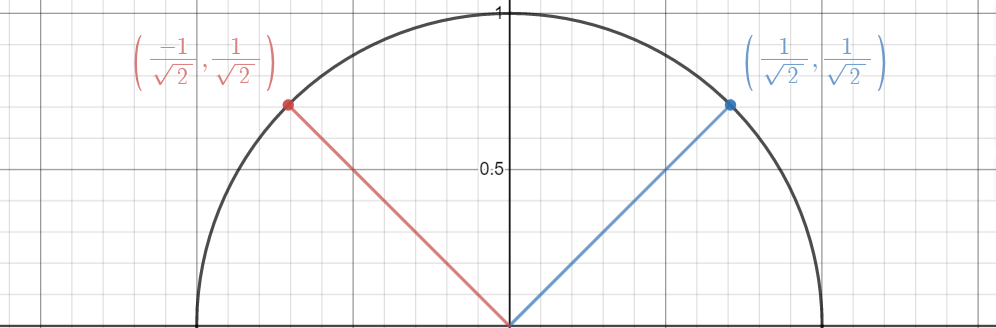
\includegraphics[width=\linewidth]{\resourceDir/img/orthonormal_bases_theta_pi_by_2.png}
			\caption{$ (\cos{\pi/4}, \sin{\pi/4})^T = (1/\sqrt{2}, 1/\sqrt{2})^T,\;  (-\sin{\pi/4}, \cos{\pi/4})^T = (-1/\sqrt{2}, 1/\sqrt{2})^T $}
		\end{figure}
		\\But for any value of the angle $\theta$ these remain orthogonal as can be seen if we generate the basis vectors for ${ \theta = \pi/3 }$.
		\begin{figure}[h!]
			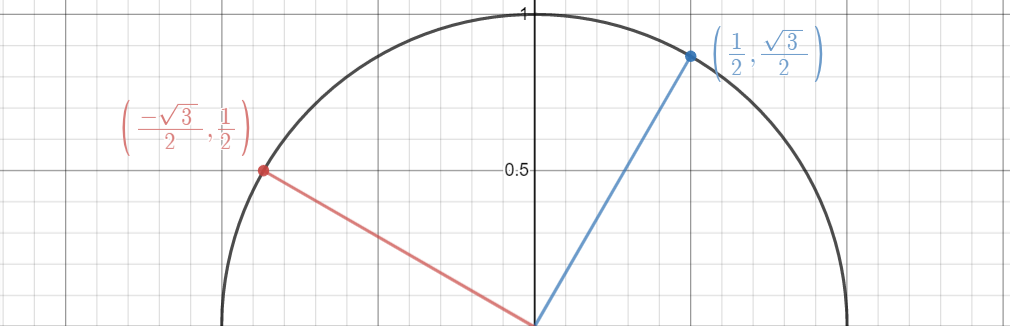
\includegraphics[width=\linewidth]{\resourceDir/img/orthonormal_bases_theta_pi_by_3.png}
			\caption{$ (\cos{\pi/3}, \sin{\pi/3})^T = (1/2, \sqrt{3}/2)^T,\;  (-\sin{\pi/3}, \cos{\pi/3})^T = (-\sqrt{3}/2, 1/2)^T $}
		\end{figure}
		\clearpage
		
		
		\subsubsection{Unitary and Orthogonal Operators}
		\bigskip
		\boxeddefinition{A matrix whose columns form an orthonormal basis is called an \textbf{orthogonal matrix}.\\\\
			The operation of left multiplication by such a matrix is called an \textbf{orthogonal operator}.
		}
		
		\bigskip
		\labeledProposition{A matrix ${ A \in \R{n \times n} }$ is orthogonal iff ${ A^T = \inv{A}}$.}{real-orthogonal-matrix-transpose-is-inverse}
		\begin{proof}
			$A$ is an orthogonal matrix so, by definition, its columns form an orthogonal basis. Then,
			\begin{align*}
				&& A^TA &=
				\begin{bmatrix}
					a_{11} & a_{21} & \cdots & a_{n1}\\
					a_{12} & a_{22} & \cdots & a_{n2}\\
					\vdots \\
					a_{1n} & a_{2n} & \cdots & a_{nn}
				\end{bmatrix}
				\begin{bmatrix}
					a_{11} & a_{12} & \cdots & a_{1n}\\
					a_{21} & a_{22} & \cdots & a_{2n}\\
					\vdots \\
					a_{n1} & a_{n2} & \cdots & a_{nn}
				\end{bmatrix} \\
				&&  &= \begin{bmatrix}
					a_{11}^2 + \cdots + a_{n1}^2 & a_{11}a_{12} + \cdots + a_{n1}a_{n2} & \cdots\\
					a_{12}a_{11} + \cdots + a_{n2}a_{n1} & a_{12}^2 + \cdots + a_{n2}^2 & \cdots\\
					\vdots \\
					\cdots & \cdots & \cdots & a_{1n}^2 + \cdots + a_{nn}^2
				\end{bmatrix}
			\end{align*}
			Along the main diagonal the components take the form
			\[ a_{1j}^2 + a_{2j}^2 + \cdots + a_{nj}^2 = a_j \dotprod a_j \]
			where ${ a_j }$ is the $j$th column of the matrix $A$. But the columns of $A$ are vectors in an orthonormal basis and so ${ a_j \dotprod a_j= 1 }$.\\
			Furthermore, the off-diagonal values take the form
			\[ a_{1j}a_{1j'} + \cdots + a_{nj}a_{nj'} = a_j \dotprod a_{j'} \]
			for ${ j \neq j' }$. Since the columns are from an orthonormal basis we know that ${ a_j \dotprod a_{j'} = 0 }$.\\
			Therefore the resultant matrix looks like,
			\[ A^TA = \begin{bmatrix}
				1 & 0 & \cdots & 0\\
				0 & 1 & \cdots & 0\\
				\vdots\\
				0 & 0 & \cdots & 1
			\end{bmatrix}
			= I_n.
			\]
			Clearly, the same effect would be seen for ${ AA^T }$ and so,
			\[ A^TA = AA^T = I \iff A^T = \inv{A}. \]
			
			Conversely, we can reverse the logic and it is easy to see that if ${ A^T A = I }$ then,
			\begin{enumerate}[label=(\roman*)]
				\item{since the diagonal entries are all 1, if $\u_i$ is a column of $A$, then ${ \u_i \dotprod \u_i = 1 }$;}
				\item{since the off-diagonal entries are all 0, if ${ \u_i, \u_j }$ with ${ i \neq j }$ are distinct columns of $A$, then  ${ \u_i \dotprod \u_j = 0 }$.}
			\end{enumerate}
			Therefore, the columns of $A$ form an orthogonal basis and thus, by definition, $A$ is an orthogonal matrix.
		\end{proof}
		
		\note{This provides another way of seeing \autoref{prop:inner-prod-of-vector-with-orthonormal-basis-vector-is-coordinate}: If $[B]$ is the matrix whose columns are the vectors of an orthonormal basis then --- just as with any change of basis --- the vector $\x$ \wrt the standard basis, has coordinates \wrt the basis $B$ given by,
			\[ \inv{[B]}\x. \]
			But, since $[B]$ is an orthogonal matrix,
			\[ \inv{[B]}\x = [B]^T\x \]
			which is the vector whose $i$-th row component is the dot product of the $i$-th column of $[B]$ and $\x$.
		}
	
		\bigskip
		\labeledProposition{A matrix ${ A \in \C{n \times n} }$ is unitary iff its columns are an orthonormal basis of $\C{n}$.}{matrix-is-unitary-iff-columns-are-orthonormal-basis}
		\begin{proof}
			Assume $A$ is a unitary matrix in  $\C{n \times n}$ and let its rows be denoted $a_i$ and its columns be denoted $a_j$, for ${ 1 \leq i,j \leq n }$. The unitary property of $A$ tells us that,
			\[ A^* A = \conj{A}^T A = I. \]
			Each row of the matrix $\conj{A}^T$ has the form $\conj{a_j}$, the conjugate of the $j$-th row of $A$. Therefore, by matrix multiplication, the diagonal entries of the matrix product $\conj{A}^T A$ are given by the expression ${ \conj{a_j} \dotprod a_j }$ while every entry off the main diagonal is given by the expression ${ \conj{a_m} \dotprod a_j }$ for some ${ m \neq j }$. Since the product is equal to the identity matrix --- which has all diagonal entries equal to 1 and all off-diagonal entries equal to 0 --- we must have, for all ${ 1 \leq m \neq j \leq n }$
			\[ \conj{a_j} \dotprod a_j = 1 \, \land \, \conj{a_m} \dotprod a_j = 0. \]
			Therefore, by \ref{def:orthonormal-set}, the columns $a_j$ are an orthonormal set. Since each columns is an $n$-vector in $\C{n}$ and there are $n$ orthonormal columns, by \ref{coro:dim-V-orthogonal-vectors-are-basis}, they are a basis of $\C{n}$.\\
			
			Conversely, assume that the columns of a matrix ${ A \in \C{n \times n} }$ are an orthonormal basis of $\C{n}$. Then, applying the logic above in reverse we have that,
			\[ A^* A = I \]
			and so $A$ is unitary. (\TODO{does this prove the inverse exists on both sides?})
		\end{proof}
		
		
		
		\bigskip
		\labeledProposition{In a real vector space, left multiplication by an orthogonal matrix preserves the dot product. In other words, for all vectors ${ \v,\w }$, $A$ is an orthogonal matrix if and only if,
			\[ A\v \dotprod A\w = \v\dotprod\w. \]
		}{left_mult_by_ortho_matrix_preserves_dot_product}
		\begin{proof}
			Using \autoref{prop:real-orthogonal-matrix-transpose-is-inverse} and the matrix formula for the dot product we can deduce that, for all vectors ${ \v,\w }$,
			\begin{align*}
				&& A\v \dotprod A\w &= (A\v)^T A\w \\
				&&  &= \v^TA^TA\w &\sidecomment{} \\
				&&  &= \v^T\w &\sidecomment{$A$ is orthogonal so ${A^TA = I}$} \\
				&&  &= \v \dotprod \w
			\end{align*}
			which is to say that an orthogonal matrix preserves the dot product.\\
			
			Conversely, if we assume that $A$ preserves the dot product then, for all vectors ${ \v,\w }$,
			\begin{align*}
				&& A\v \dotprod A\w &= \v \dotprod \w  \\
				&\iff & (A\v)^TA\w &= \v^T\w & \\
				&\iff & \v^TA^TA\w &= \v^T\w & \\
				&\iff & \v^TA^TA\w - \v^T\w &= 0 & \sidecomment{both terms are scalars}\\
				&\iff & \v^T(A^TA - I)\w &= 0. &
			\end{align*}
			Now for any arbitrary matrix $B$, 
			\[ \e{i}^T B \e{j} = b_{ij} \]
			where $b_{ij}$ is the $(i,j)$th element of $B$. Then, for
			\[ \e{i}^T B \e{j} = 0 \]
			to be true \textit{for all possible} ${ \e{i},\e{j} }$ would require that, 
			\[ \forall i,j \logicsep b_{ij} = 0 \iff B = [0] \]
			where $[0]$ is the zero matrix. Therefore,
			\[ \forall \v,\w \logicsep \v^T(A^TA - I)\w = 0 \iff A^TA - I = [0] \iff A^TA = I \]
			which, by \autoref{prop:real-orthogonal-matrix-transpose-is-inverse}, implies that $A$ is orthogonal. So if $A$ preserves the dot product then it is orthogonal.
		\end{proof}
	
		\bigskip
		\labeledProposition{A matrix ${ A \in \C{n \times n} }$ is unitary iff it preserves the standard complex inner product. That's to say,
			\[ \forall \x,\y \in \C{n} \logicsep (A \x)^* A \y = \x^* \y.  \]
		}{matrix-is-unitary-iff-preserves-the-standard-complex-inner-product}
		\begin{proof}
			If we assume that $A$ is unitary then, by properties of the hermitian conjugate (\ref{def:hermitian-conjugate}),
			\[ (A\x)^* A\y = \x^* (A^* A) \y = \x^* \y \]
			which shows that $A$ preserves the standard complex inner product.\\
			
			\note{A possible alternative proof?\\\\
				Conversely, if we assume that $A$ preserves the standard complex inner product then,
				\[\begin{aligned}
					&& (A \x)^* A \y &= \x^* \y \\
					&\iff & \x^* (A^* A) \y &= \x^* \y &\sidecomment{by hermitian conjugate properties} \\
					&\iff & \x^* (A^* A) \y &= \x^* I \y.
				\end{aligned}\]
				and this implies, by \ref{prop:quadratic-forms-equal-for-all-vectors-in-space-implies-matrices-are-equal}, that ${ A^* A = I }$. This therefore shows that $A$ is unitary. (\TODO{does this prove the inverse exists on both sides?})
			}
			
			Conversely, if we assume that $A$ preserves the standard complex inner product then,
			\[ \forall \x,\y \in \C{n} \logicsep (A \x)^* A \y = \x^* \y. \]
			Since this applies to all vectors in $\C{n}$, it must apply to the standard basis vectors of $\C{n}$,
			\[ (A \e{p})^* A \e{q} = {a_p}^* a_q = \e{p}^* \e{q} \]
			where $a_i$ denotes the $i$-th column of the matrix $A$. Since the expression ${ \e{p}^* \e{q} }$ is 0 for all ${ p \neq q }$ and 1 for ${ p = q }$ we deduce that the columns of $A$ are such that ${ {a_p}^* a_q }$ is 0 for all ${ p \neq q }$ and 1 for ${ p = q }$. The columns of $A$ are, therefore, an orthonormal set and so also an orthonormal basis of $\C{n}$. It follows then, that $A$ is unitary.
		\end{proof}
		
		
		\bigskip
		\labeledProposition{The determinant of any orthogonal matrix is 1 or -1.}{determinant_of_orthogonal_matrix}
		\begin{proof}
			If a matrix $A$ is orthogonal then ${ A^TA = I }$ which implies that,
			\[ det(A^T)det(A) = det(I) = 1. \]
			By \autoref{prop:determinant_of_matrix_equal_to_its_transpose}, ${ det(A^T) = det(A) }$ so,
			\[ det(A^T)det(A) = det(A)^2 = 1 \iff \sqrt{det(A)} = 1 \iff det(A) = \pm 1.  \qedhere \]
		\end{proof}
		
		\note{If an orthogonal operator has determinant equal to 1 it is described as \textbf{orientation preserving} and if it is equal to -1 it is described as \textbf{orientation reversing}.}
		
		\bigskip
		\labeledProposition{The orthogonal matrices form a subgroup of $GL_n(\F{})$.}{orthogonal-matrices-are-subgroup}
		\begin{proof}
			Let ${ S = \setc{ A \in GL_n(\F{}) }{ A^TA = I } }$. Then,
			\begin{itemize}
				\item{$S$ is nonempty because ${ I \in S }$.}
				\item{For ${ B,C \in S }$,
					\[ (BC)^T(BC) = C^TB^T(BC) = C^T(B^TB)C = I \]
					so ${ BC \in S }$.
				}
				\item{For ${ B \in S }$, by \autoref{prop:real-orthogonal-matrix-transpose-is-inverse}, ${ \inv{B} = B^T }$ and
					\[ (B^T)^TB^T = BB^T = B\inv{B} = I \]
					so $S$ contains inverses.
				}
			\end{itemize}
			Therefore ${ S \leq GL_n(\F{}) }$.	
		\end{proof}
		
		\medskip
		\note{The subgroup of the general linear group formed by the orthogonal matrices is called the \textbf{orthogonal group} and is denoted $O_n$.}
		
		

		
		
		\biggerskip
		\subsubsubsection{Example}
		\begin{exe}
			\ex{The matrix
				\[
				P = \begin{bmatrix}
					\frac{1}{\sqrt{2}} & \frac{i}{\sqrt{2}}\nn
					\frac{i}{\sqrt{2}} & \frac{1}{\sqrt{2}}
				\end{bmatrix} =
				\frac{1}{\sqrt{2}}
				\begin{bmatrix}
					1 & i\\
					i & 1
				\end{bmatrix}
				\]
				is a unitary matrix because
				\[
				P^* = 	\frac{1}{\sqrt{2}}
				\begin{bmatrix}
					1 & -i\\
					-i & 1
				\end{bmatrix}
				\]
				so that 
				\[ 
				P P^* = \frac{1}{2}
				\begin{bmatrix}
					1 & i\\
					i & 1
				\end{bmatrix}
				\begin{bmatrix}
					1 & -i\\
					-i & 1
				\end{bmatrix} = I.
				\]
				
				\nl Note that $P$ is not a hermitian matrix (\ref{def:hermitian-matrix}), but would be if one of the diagonal values were multiplied by -1, e.g. the matrix
				\[ 
				Q = \begin{bmatrix}
					\frac{1}{\sqrt{2}} & -\frac{i}{\sqrt{2}}\nn
					\frac{i}{\sqrt{2}} & \frac{1}{\sqrt{2}}
				\end{bmatrix} =
				\frac{1}{\sqrt{2}}
				\begin{bmatrix}
					1 & -i\\
					i & 1
				\end{bmatrix}
				\]
				is hermitian because ${ Q^* = Q }$.
			}
		\end{exe}
		
		
		\biggerskip
		\subsubsection{Gram-Schmidt Orthonormalisation}\label{sssection:gram-schmidt-orthonormalisation}
		\boxeddefinition{The process known as \textbf{Orthonormalisation} takes a set of linearly independent vectors and returns an orthonormal set of the same cardinality as the original set and in the same space spanned by the original set.\\ Since the orthonormal set has the same cardinality as the original set, by \autoref{coro:dim-V-orthogonal-vectors-are-basis}, it is an orthonormal basis for the space spanned by the original set.}
		
		\biggerskip
		The Gram-Schmidt algorithm is as follows:
		\begin{algorithm}
			\begin{algorithmic}
				\REQUIRE A $k$-length linearly independent set of vectors ${ S = \{\v_1,\dots,\v_k\} \subset V }$ where $V$ is an inner product space, and an initially-empty set ${ O = \{\} }$.
				\ENSURE A $k$-length orthonormal set of vectors ${ O = \{\u_1, \dots, \u_k \} }$ \suchthat ${ \operatorname{Lin} O = \operatorname{Lin} S }$.
				\STATE % empty line
				\FOR {$i=1$ to $k$}
				\STATE find $\w$, a basis for the orthogonal complement of $O$ in ${ O \cup \{\v_i\} }$.
				\STATE ${ \u_i \leftarrow \frac{\w}{\norm{\w}} }$
				\ENDFOR 
			\end{algorithmic}	
		\end{algorithm}
		% Note: This article: https://www.math-linux.com/latex-26/faq/latex-faq/article/how-to-write-algorithm-and-pseudocode-in-latex-usepackage-algorithm-usepackage-algorithmic says, at the end, that the algorithmic package used here is not compatible with hyperref.
		
		
		\medskip
		The process of finding the orthogonal complement on iteration number $i$ is to find the set of vectors
		\[ O^\perp = \setc{\w \in O \cup \{\v_i\}}{\forall \u \in O \logicsep \w \perp \u}. \]
		
		For ${ \w \in O^\perp }$ we need, for every ${ \u_j \in O }$,
		\[\begin{aligned}
			&& \inner{\w}{\u_j} &= 0 \\
			&\iff & \inner{\alpha_1 \u_1 + \cdots + \alpha_{i-1} \u_{i-1} + \alpha_i \v_i}{\u_j} &= 0 \\
			&\iff & \inner{\alpha_j \u_j + \alpha_i \v_i}{\u_j} &= 0 &\sidecomment{by orthogonality} \\
			&\iff & \alpha_j + \alpha_i \inner{\v_i}{\u_j}  &= 0 &\sidecomment{${ \because \norm{\u_j} = 1 }$} \\
			&\iff & \alpha_j &= -\alpha_i \inner{\v_i}{\u_j}.
		\end{aligned}\]
		So, if we set ${ \alpha_i = 1 }$ then we get
		\[ \w = \v_i - \inner{\v_i}{\u_1}\u_1 - \inner{\v_i}{\u_2}\u_2 - \cdots - \inner{\v_i}{\u_{i-1}}\u_{i-1}. \]
		Clearly, our only degree of freedom in the definition of the vector $\w$ is the value of $\alpha_i$. However, if we were to use some other value, ${ \alpha_i = \beta }$, then the result would be ${ \beta \w }$, a scaling of $\w$ by $\beta$. As a result, this is clearly a 1-dimensional space in which any vector will suffice as a basis. So we can use $\w$ as the basis vector and then, it is a simple matter to normalize it and add it to the set $O$.
		
		
		

		
		
		
		\biggerskip
		\subsubsection{Unitary and Orthogonal Diagonalisation}
		\bigskip
		\boxeddefinition{\textbf{(Unitary Diagonalisation)} A matrix is said to be \textit{unitarily diagonalisable} if there is a unitary matrix that diagonalises it. That's to say, the matrix $A$ is unitarily diagonalisable iff there exists some unitary matrix $P$ such that
			\[ P^* A P = D \]
			is diagonal.\\
			
			Note that since $P$ is unitary (\ref{def:unitary-matrix}), this definition implies the non-unitary diagonlisation condition,
			\[ P^* A P = \inv{P} A P = D \]
			with the difference being that, for the diagonalising matrix $P$,
			\[ \inv{P} = \conj{P}^T = P^*. \]
		}\label{def:unitary-diagonalisation}
		\boxeddefinition{\textbf{(Orthogonal Diagonalisation)} A real matrix is said to be \textit{orthogonally diagonalisable} if there is an orthogonal matrix that diagonalises it. That's to say, the matrix $A$ is orthogonally diagonalisable iff there exists some real orthogonal matrix $P$ such that
			\[ \inv{P} A P = P^T A P = D \]
			is diagonal.
		}\label{def:orthogonal-diagonalisation}
		
		
		\bigskip
		\labeledProposition{The matrix ${ A \in \C{n \times n} }$ is unitarily diagonalisable iff there exists an orthonormal eigenbasis of $A$.}{matrix-is-unitarily-diagonalisable-iff-exists-eigenvec-basis-of-complex-space}
		\begin{proof}
			If the matrix $A$ is unitarily diagonalisable then there exists a unitary matrix ${ P \in \C{n \times n} }$ such that,
			\[ D = P^* A P = \inv{P} A P \]
			is diagonal. This implies that the columns of $P$ are an eigenbasis for the matrix $A$ (\ref{def:eigenbasis}) and, since $P$ is unitary, by \autoref{prop:matrix-is-unitary-iff-columns-are-orthonormal-basis}, the columns are also an orthonormal basis of $\C{n}$.\\
			
			Conversely, if there exists an orthonormal basis of $\C{n}$ consisting solely of eigenvectors of $A$ then there exists a matrix ${ P \in \C{n \times n} }$ whose columns are the vectors of this basis. Then by the definition of the eigenbasis \ref{def:eigenbasis},
			\[ D = \inv{P} A P \]
			is diagonal. Since the columns of $P$ are an orthonormal basis, then $P$ is unitary and so we have,
			\[ D = \inv{P} A P = P^* A P \]
			which is the property for $A$ to be unitarily diagonalisable.
		\end{proof}
		\begin{corollary}
			A real matrix is orthogonally diagonalisable iff there exists an orthonormal eigenbasis of $A$.
		\end{corollary}
		\begin{proof}
			This is a special case of \autoref{prop:matrix-is-unitarily-diagonalisable-iff-exists-eigenvec-basis-of-complex-space}. If the matrix ${ A \in \C{n \times n} }$ has only real-valued entries then we also have ${ A \in \R{n \times n} \subset \C{n \times n} }$. In this case, orthogonal diagonalisability means that there is a real orthogonal matrix that diagonlises $A$, which implies that there is an orthonormal set of eigenvectors of $A$ that forms a basis of $\R{n}$.\\
			Conversely, if there exists an orthonormal eigenbasis for $A$ in $\R{n}$ then there is a diagonalising matrix whose columns are this orthonormal basis and the matrix will therefore be orthogonal.
		\end{proof}
	
	
	
		\bigskip
		\labeledProposition{The eigenvectors corresponding to distinct eigenvalues of a Hermitian matrix are orthogonal \wrt to the standard inner product.}{hermitian-matrix-eigenvectors-for-distinct-eigenvalues-are-orthogonal}
		\begin{proof}
			Let $A$ be a hermitian matrix (\ref{def:hermitian-matrix}). Let $\lambda_1$ and $\lambda_2$ be distinct eigenvalues of $A$ and let $\v_1$ be an eigenvector corresponding to $\lambda_1$ and $\v_2$ an eigenvector corresponding to $\lambda_2$. Then,
			\[\begin{aligned}
				&& \v_1^* A \v_2 &= \v_1^* A^* \v_2     &\sidecomment{$\because A$ is hermitian}\\
				&\iff & \v_1^* (A \v_2) &= (A \v_1)^* \v_2     &\sidecomment{by props. of hermitian conjugate \ref{def:hermitian-conjugate}} \\
				&\iff & \v_1^* (\lambda_2 \v_2) &= (\lambda_1 \v_1)^* \v_2    &\sidecomment{by eigenvalue property} \\
				&\iff & \v_1^* \lambda_2 \v_2 &= \conj\lambda_1 \v_1^* \v_2    &\sidecomment{by \ref{prop:hermitian-conj-of-scalar-x-matrix-is-conj-of-scalar-x-hermitian-conj-of-matrix}} \\
				&\iff & \lambda_2 \v_1^* \v_2 &= \lambda_1 \v_1^* \v_2    &\sidecomment{by \ref{prop:hermitian-matrix-has-only-real-eigenvalues}} \\
				&\iff & (\lambda_2 - \lambda_1) \v_1^* \v_2 &= 0 \\
				&\therefore & \v_1^* \v_2 &= 0.   &\sidecomment{${ \because \lambda_1 \neq \lambda_2 \implies \lambda_2 - \lambda_1 \neq 0 }$}
			\end{aligned}\]
			This last result says that the standard complex inner product of $\v_1$ and $\v_2$ is zero, which is to say that $\v_1$ and $\v_2$ are orthogonal \wrt to the standard complex inner product.
		\end{proof}
		\TODO{does this result imply that the eigenvectors are orthogonal \wrt every basis and every inner product or only the standard basis and inner product?}
		
	
	
		\bigskip
		\labeledProposition{A normal matrix is hermitian iff it has only real-valued eigenvalues.}{normal-matrix-is-hermitian-iff-only-has-real-eigenvals}
		\begin{proof}
			Let $A$ be a normal matrix with only real-valued eigenvalues. By \autoref{prop:matrix-is-unitarily-diagonalisable-iff-normal}, $A$ is unitarily diagonalisable so there exists a unitary matrix $P$ such that,
			\[ D = P^* A P \]
			is a diagonal matrix whose diagonal entries are the eigenvalues of $A$. Since, by hypothesis, these are all real numbers, we have ${ D^* = D }$. Using this fact and the rearranged relation with the diagonal matrix ${ A = P D P^* }$,
			\[\begin{aligned}
				A^* &= (P D P^*)^* \\
				&= P D^* P^* &\sidecomment{by props. of hermitian conjugate \ref{def:hermitian-conjugate}} \\
				&= P D P^* = A.
			\end{aligned}\]
			
			Conversely, let $A$ be a hermitian matrix (\ref{def:hermitian-matrix}) and let $\lambda$ be an arbitrary eigenvalue of $A$ with $\v$ as an eigenvector corresponding to $\lambda$. Then,
			\[\begin{aligned}
				&& \v^* A \v &= \v^* A^* \v   &\sidecomment{${ \because A }$ is hermitian}\\
				&\iff & \v^* (A \v) &= (A \v)^* \v   &\sidecomment{by props. of hermitian conjugate \ref{def:hermitian-conjugate}} \\
				&\iff & \v^* (\lambda \v) &= (\lambda \v)^* \v   &\sidecomment{by eigenvalue property}\\
				&\iff & \v^* (\lambda \v) &= \conj\lambda \v^* \v   &\sidecomment{by \ref{prop:hermitian-conj-of-scalar-x-matrix-is-conj-of-scalar-x-hermitian-conj-of-matrix}}\\
				&\iff & \lambda \norm{\v}^2 &= \conj\lambda \norm{\v}^2   &\sidecomment{by defn. of induced norm \ref{def:vector-norm}} \\
				&\iff & \lambda &= \conj\lambda   &\sidecomment{${ \because \v \neq \0 \implies \norm{\v} > 0 }$ so has inverse} \\
				&\therefore & \lambda &\in \R{}.  \qedhere
			\end{aligned}\]
		\end{proof}
		\begin{corollary}
			A real symmetric matrix has only real-valued eigenvalues.
		\end{corollary}
		\begin{proof}
			This follows from \autoref{prop:normal-matrix-is-hermitian-iff-only-has-real-eigenvals} and the fact that for a symmetric matrix ${ A \in \R{n \times n} \subset \C{n \times n} }$, the operation of complex conjugation on the real entries of $A$ has no effect so that ${ \conj{A} = A }$ and, by the symmetric property, we have ${ A^T = A }$. So, putting these together we obtain,
			\[ A^* = \conj{A}^T = A^T = A \]
			which says that if $A$ is real and symmetric, then it is hermitian.
		\end{proof}
	
		
		\bigskip
		\labeledProposition{A matrix is unitarily diagonalisable iff it is normal.}{matrix-is-unitarily-diagonalisable-iff-normal}
		\begin{proof}
			If a matrix $A$ is unitarily diagonalisable then there exists a unitary matrix $P$ such that
			\[ D = P^* A P \]
			is diagonal. Then it also follows that ${ A = P D P^* }$ and so,
			\[\begin{aligned}
				A A^* &= (P D P^*) \, (P D P^*)^* \\
				&= P D P^* \, P D^* P^* &\sidecomment{} \\
				&= P D D^* P^* &\sidecomment{${ \because P \text{ is unitary } }$} \\
				&= P D^* D P^* &\sidecomment{${ \because D \text{ is diagonal } \implies D \text{ is normal }  }$} \\
				&= P D^* P^* \, P D P^* &\sidecomment{${ \because P \text{ is unitary } }$} \\
				&= (P D P^*)^* \, (P D P^*) = A^* A.
			\end{aligned}\]
			
			Conversely, assume that a matrix $A$ is normal. By the Schur decomposition (\autoref{theo:schur-decomposition}), we can write any matrix as ${ U T U^* }$, where $U$ is unitary and $T$ is upper-triangular. Letting ${ A = U T U^* }$ and using the normal property gives,
			\[\begin{aligned}
				&& A A^* &= A^* A \\
				&\iff & (U T U^*) \, (U T U^*)^* &= (U T U^*)^* \, (U T U^*) &\sidecomment{} \\
				&\iff & U T U^* \, U T^* U^* &= U T^* U^* \, U T U^* &\sidecomment{} \\
				&\iff & U T T^* U^* &= U T^* T U^* &\sidecomment{${ \because U \text{ is unitary } }$} \\
				&\iff & T T^* &= T^* T.
			\end{aligned}\]
			So the upper-triangular matrix $T$ is also normal. By \autoref{prop:normal-upper-triangular-matrix-is-diagonal} then, $T$ is diagonal. Therefore,
			\[ U^* A U = T \]
			is diagonal and $A$ is unitarily diagonalisable.
		\end{proof}
		\begin{corollary}
			A real matrix is orthogonally diagonalisable iff it is symmetric.
		\end{corollary}
		\begin{proof}
			If a matrix $A$ is orthogonally diagonalisable then there exists an orthogonal matrix $P$ such that,
			\[ D = \inv{P}AP \]
			is diagonal. Since the matrix $D$ is diagonal, it is symmetrical and equal to its transpose so we can reason,
			\[ D^T = D \implies (\inv{P}AP)^T = \inv{P}AP. \]
			Furthermore, $P$ is an orthogonal matrix so, by \autoref{prop:real-orthogonal-matrix-transpose-is-inverse}, ${ P^T = \inv{P} }$. Therefore,
			\[\begin{aligned}
				&& (\inv{P}AP)^T &= \inv{P}AP \\
				&\iff & P^T A^T (\inv{P})^T &= \inv{P}AP \\
				&\iff & \inv{P} A^T (P^T)^T &= \inv{P}AP \\
				&\iff & \inv{P} A^T P &= \inv{P}AP \\
				&\iff & A^T &= A
			\end{aligned}\]
			and $A$ is symmetric.\\			
			
			Conversely, let $A$ be a real symmetric matrix in complex space. Since $A$ is real and symmetric, it is hermitian and normal (\autoref{prop:real-symmetric-matrices-are-hermitian}, \autoref{prop:common-classes-of-normal-matrices}). The hermitian property of $A$ implies, by \autoref{prop:normal-matrix-is-hermitian-iff-only-has-real-eigenvals}, that all its eigenvalues are real-valued. The normal property of $A$, by \autoref{prop:matrix-is-unitarily-diagonalisable-iff-normal}, implies that it is unitarily diagonalisable; that's to say there exists a unitary matrix $U$ and a diagonal matrix $D$ such that,
			\[ U^* A U = D. \]
			Since all the eigenvalues of $A$ are real, by \autoref{prop:for-real-matrix-in-complex-space-a-real-eigenvalue-has-real-eigenvectors}, we can choose real eigenvectors corresponding to them. So, by construction, $U$ is real. Since $U$ is real and unitary, it is orthogonal (\autoref{prop:real-unitary-matrix-is-orthogonal}). Therefore $A$ is orthogonally diagonalisable.
		\end{proof}


		
		
		
		\sep
		\begin{exe}
			\item{The matrix
				\[ 
				A = \begin{bmatrix}
					1 & 2 + i\\
					2 - i & 5
				\end{bmatrix} 
				\]
				is hermitian and therefore also normal and so can be unitarily diagonalised. The characteristic polynomial is
				\[ \lambda^2 - 6\lambda + 5 - 5 = \lambda^2 - 6\lambda = \lambda(\lambda - 6) = 0 \]
				so the eigenvalues are ${ \lambda \in \{0, 6\} }$. Note that, as predicted by \autoref{prop:hermitian-matrix-has-only-real-eigenvalues}, the eigenvalues ae real. After row-reduction the determined eigenvectors are:
				\begin{itemize}
					\item{For ${ \lambda_1 = 0 }$,
						\[ \v_1 =  \begin{bmatrix}2 + i\\ -1 \end{bmatrix}. \]
					}
					\item{For ${ \lambda_2 = 6 }$,
						\[ \v_2 =  \begin{bmatrix}2 + i\\ 5 \end{bmatrix}. \]
					}
				\end{itemize}
				The vectors $\v_1$ and $\v_2$ are orthogonal \wrt the standard complex inner product. Their norms are $\sqrt{6}$ and $\sqrt{30}$ respectively so that the associated unitary matrix is
				\[
				P = \begin{bmatrix}
					\frac{2 + i}{\sqrt{6}} & \frac{2 + i}{\sqrt{30}} \nn
					\frac{-1}{\sqrt{6}} & \frac{5}{\sqrt{30}}
				\end{bmatrix} 
				\]
				and
				\[
				P^* A P = 	\begin{bmatrix}
					\frac{2 - i}{\sqrt{6}} & \frac{-1}{\sqrt{6}} \nn
					\frac{2 - i}{\sqrt{30}} & \frac{5}{\sqrt{30}}
				\end{bmatrix}
				\begin{bmatrix}
					1 & 2 + i\\
					2 - i & 5
				\end{bmatrix}
				\begin{bmatrix}
					\frac{2 + i}{\sqrt{6}} & \frac{2 + i}{\sqrt{30}} \nn
					\frac{-1}{\sqrt{6}} & \frac{5}{\sqrt{30}}
				\end{bmatrix} =
				\begin{bmatrix}
					0 & 0\\
					0 & 6
				\end{bmatrix}.
				\]
			}
		\end{exe}
	
		
		\biggerskip
		\subsubsection{Spectral Decomposition}
		\bigskip
		\boxeddefinition{\textbf{(Spectral Decomposition)} If an operator on a finite-dimensional inner product space is normal (\ref{def:normal-matrix}) then it can be written as a linear combination of pairwise orthogonal projections, called its \textit{spectral decomposition} or \textit{eigendecomposition}.\\
		
		The spectral decomposition is a special case of both the Schur Decomposition (\autoref{theo:schur-decomposition}) and the \href{https://en.wikipedia.org/wiki/Singular_value_decomposition}{Singular Value Decomposition}.
		}	
	
		\medskip
		\labeledTheorem{\textbf{(Spectral Decomposition)} Let $A$ be a normal matrix and let ${ \{\x_1,\x_2,\dots,\x_n\} }$ be an orthonormal basis of eigenvectors of $A$ with corresponding eigenvalues ${ \{\lambda_1,\lambda_2,\dots,\lambda_n\} }$. Then,
			\[ A = \lambda_1 \x_1 \x_1^* + \lambda_2 \x_2 \x_2^* + \cdots + \lambda_n \x_n \x_n^*. \]
		}{spectral-decomposition}
		\begin{proof}
			Let
			\[ B = \lambda_1 \x_1 \x_1^* + \lambda_2 \x_2 \x_2^* + \cdots + \lambda_n \x_n \x_n^*. \]
			For each eigenvalue $\lambda_i$ of $A$ with associated eigenvector $\x_i$,
			\[\begin{aligned}
				&& A\x_i &= B\x_i \\
				&\iff & \lambda_i \x_i &= (\lambda_1 \x_1 \x_1^* + \cdots + \lambda_n \x_n \x_n^*)\x_i \\
				&\iff & \lambda_i \x_i &= (\lambda_i \x_i \x_i^*)\x_i &\sidecomment{${ \because \forall i \neq j \logicsep \x_i \perp \x_j \implies \x_j^* \x_i = 0 }$} \\
				&\iff & \lambda_i \x_i &= (\lambda_i \x_i) \norm{\x_i}^2 \\
				&\iff & \lambda_i \x_i &= \lambda_i \x_i.
			\end{aligned}\]
			This result implies that the expression $B$ is a matrix that has the same eigenvalues and corresponding eigenvectors as $A$. Therefore, by diagonalisability of $A$ and \autoref{prop:diagonalisable-matrices-with-same-eigenvals-and-eigenvecs-are-equal}, ${ A = B }$.
		\end{proof}
	
		\bigskip
		\labeledProposition{Let $A$ be a normal matrix and let
			\[ A = \lambda_1 \x_1 \x_1^* + \lambda_2 \x_2 \x_2^* + \cdots + \lambda_n \x_n \x_n^* \]
			be the spectral decomposition of $A$. Then each ${ \x_i \x_i^* }$ is an ${ n \times n }$ matrix representing pairwise orthogonal projections onto the respective eigenspace of the eigenvalue $\lambda_i$.
		}{spectral-decomposition-produces-orthogonal-projections-onto-the-eigenspaces}
		\begin{proof}
			\begin{itemize}
				\item{Each matrix $\x_i \x_i^*$ is real and symmetric which implies that they are hermitian.}
				\item{Mutual orthogonality \wrt standard complex inner product is easy to show.}
				\item{
					\[ (\x_i \x_i^*)(\x_i \x_i^*) \v = \x_i (\x_i^* \x_i) \x_i^* \v = \x_i (1) \x_i^* \v = \x_i \x_i^* \v \]
					means that they are idempotent.
				}
				\item{These properties imply that they are orthogonal projections.}
				\item{They clearly project onto the associated eigenspace because the eigenvectors $\x_i$ are an eigenbasis so that for any $\v$ in the space,
					\[ \v = \alpha_1 \x_1 + \cdots + \alpha_n \x_n \]
					and so the action of a matrix $\x_i \x_i^*$ on a vector in the space is,
					\[ x_i \x_i^* \v = x_i \x_i^* (\alpha_1 \x_1 + \cdots + \alpha_n \x_n) = \x_i \x_i^* \alpha_i \x_i = \alpha_i \x_i. \]
				}
			\end{itemize}
			\TODO{complete this after studying orthogonal projections}
		\end{proof}
	
		
		\bigskip
		\labeledProposition{If matrices ${ E_1,E_2,\dots,E_n }$ are orthogonal projections then, for any real scalars ${ \alpha_1,\alpha_2,\dots,\alpha_n }$ and any positive integer $m$,
			\[ (\alpha_1 E_1 + \alpha_2 E_2 + \cdots + \alpha_n E_n)^m = \alpha_1^m E_1 + \alpha_2^m E_2 + \cdots + \alpha_n^m E_n. \]
		}{product-of-a-sum-of-orthogonal-projections-has-no-cross-terms}
		\begin{proof}
			\TODO{proof}
		\end{proof}
	
	
	}

	
% -------------------- break ------------------
\pagebreak

		
		\searchableSubsection{Quadratic Forms}{linear algebra}{
			\bigskip
			\boxeddefinition{\textbf{(Quadratic Form)} A \textit{quadratic form} in ${ n \geq 2 }$ variables is a polynomial over the reals in which every term has degree 2 in the variables.\\
				In matrix form, a quadratic form $q$ is an expression,
				\[ q = \x^T A \x \]
				where ${ A \in \R{n \times n} }$ is symmetric and ${ \x \in \R{n} }$.
			}
		
			\bigskip
			\labeledProposition{A matrix is positive definite iff all its principal minors (\ref{def:principal-minors}) are positive.}{matrix-is-positive-definite-iff-all-principal-minors-are-positive}
			\begin{proof}
				see Artin[252-262].
			\end{proof}
		
			\bigskip
			\labeledProposition{A matrix is positive negative iff its principal minors (\ref{def:principal-minors}) of odd order are negative and those of even order are positive.}{matrix-is-negative-definite-iff-sign-of-principal-minors-alternates}
			\begin{proof}
				see Artin[252-262].
			\end{proof}
		
			\bigskip
			\note{Note that there is no simple check for positive or negative semi-definiteness (see example \ref{ex:principal-minors-check-indeterminate-case}).}
			
			\bigskip
			\labeledProposition{Let ${ A \in \F{m \times n} }$ be a matrix with full column rank (i.e. ${ \operatorname{rank} A = n }$ defined in an inner product space equipped with the standard complex inner product (\ref{def:inner-product}). Then ${ A^* A }$ is:
				\begin{enumerate}[label=(\roman*)]
					\item{Hermitian,}
					\item{Invertible.}
				\end{enumerate}
			}{properties-of-full-column-rank-matrix-product-with-hermitian-conjugate}
			\begin{proof}\nl
				\begin{enumerate}[label=(\roman*)]
					\item{${ (A^* A)^* = A^* A }$}
					\item{
						\subheading{alternative proof 1}
						Let 
						\[ A^* A \x = \0 \implies A\x \in N(A^*). \]
						By, \autoref{prop:matrix-nullspace-is-orthogonal-complement-of-range-of-hermitian-conjugate}, we have
						\[ N(A^*) = R((A^*)^*)^\perp = R(A)^\perp. \]
						That's to say, the nullspace of $A^*$ is the orthogonal complement of the range of $A$. Therefore, 
						\[ A\x \in N(A^*) \iff A\x \in R(A)^\perp. \]
						But ${ R(A) = \setc{A\v}{\v \in \F{n}} }$ so also ${ A\x \in R(A) }$. It follows then that 
						\[ A\x \in R(A) \cap R(A)^\perp. \]
						By \autoref{prop:vector-orthogonal-complement-is-complement-space}, 
						\[ R(A) \oplus R(A)^\perp = \F{m} \implies R(A) \cap R(A)^\perp = \{\0\} \]
						so
						\[ A\x = \0. \]
						But, by hypothesis, $A$ is full column rank and so
						\[ A\x = \0 \iff \x = \0. \]
						
						\subheading{alternative proof 2}
						Let 
						\[ \x \in N(A^* A) \implies A^* A \x = \0. \]
						Then,
						\[ \x^* A^* A \x = 0 = (A\x)^* A\x = \inner{A\x}{A\x} = \norm{A\x}^2. \]
						Then, the positive definiteness property of the inner product allows us to deduce that
						\[ \norm{A\x}^2 = 0 \implies A\x = 0 \implies \x \in N(A). \]
						But $A$ has full column rank and so ${ N(A) = \{\0\} }$ which implies that ${ \x = \0 }$.\\
						
						\subheading{conclusion}
						Since we have shown that
						\[ A^* A \x = \0 \implies \x = \0 \]
						it follows that
						\[ N(A^* A) = \{\0\} \]
						which, by \autoref{coro:linear-transformation-is-injective-iff-kernel-is-trivial}, implies that ${ A^* A }$ is invertible.
					}
				\end{enumerate}
			\end{proof}
			\begin{corollary}\label{coro:properties-of-real-full-column-rank-matrix-product-with-transpose}
				Let ${ A \in \R{m \times n} }$ be a real matrix with full column rank (i.e. ${ \operatorname{rank} A = n }$). Then ${ A^T A }$ is:
				\begin{enumerate}[label=(\roman*)]
					\item{Positive definite;}
					\item{Symmetric;}
					\item{Invertible.}
				\end{enumerate}
			\end{corollary}
			\begin{proof}
				\TODO{prove this}
			\end{proof}
			
			
			\sep
			\begin{exe}
				\ex{
					Let
					\[
						A = \begin{bmatrix}
								1 & 1 & 0\\
								1 & 1 & 0\\
								0 & 0 & t
							\end{bmatrix}.
					\]
					The eigenvalues of $A$ are ${ \lambda \in \{ 0,2,t \} }$. The principal minors of $A$ are
					\[
						a_{11} = 1, \hspace{20pt} \begin{vmatrix}1 & 1\\ 1 & 1\end{vmatrix} = 0, \hspace{20pt} \det{A} = 0.
					\]
				}\label{ex:principal-minors-check-indeterminate-case}
			\end{exe}
		}
	
\end{document}